\documentclass[a4paper,twoside]{article}
\usepackage[T1]{fontenc}
\usepackage[bahasa]{babel}
\usepackage{graphicx}
\usepackage{graphics}
\usepackage{float}
\usepackage[cm]{fullpage}
\pagestyle{myheadings}
\usepackage{etoolbox}
\usepackage{setspace} 
\usepackage{lipsum} 
\usepackage{listings}
\setlength{\headsep}{30pt}
\usepackage[inner=2cm,outer=2.5cm,top=2.5cm,bottom=2cm]{geometry} %margin
% \pagestyle{empty}
\usepackage{graphicx}%untuk graphicspath
\graphicspath{ {./images/} }
\usepackage[obeyspaces,spaces]{url}

\makeatletter
\renewcommand{\@maketitle} {\begin{center} {\LARGE \textbf{ \textsc{\@title}} \par} \bigskip {\large \textbf{\textsc{\@author}} }\end{center} }
\renewcommand{\thispagestyle}[1]{}
\markright{\textbf{\textsc{Laporan Perkembangan Pengerjaan Skripsi\textemdash Sem. Gajil 2019/2020}}}

\onehalfspacing
 
\begin{document}

\title{\@judultopik}
\author{\nama \textendash \@npm} 

%ISILAH DATA BERIKUT INI:
\newcommand{\nama}{Muhammad Ravi}
\newcommand{\@npm}{2016730041}
\newcommand{\tanggal}{21/11/2019} %Tanggal pembuatan dokumen
\newcommand{\@judultopik}{Studi dan Implementasi Spark Streaming untuk Mengumpulkan Big Data Stream} % Judul/topik anda
\newcommand{\kodetopik}{VSM4702}
\newcommand{\jumpemb}{1} % Jumlah pembimbing, 1 atau 2
\newcommand{\pembA}{Veronica Sri Moertini}
\newcommand{\pembB}{-}
\newcommand{\semesterPertama}{47 - Ganjil 19/20} % semester pertama kali topik diambil, angka 1 dimulai dari sem Ganjil 96/97
\newcommand{\lamaSkripsi}{1} % Jumlah semester untuk mengerjakan skripsi s.d. dokumen ini dibuat
\newcommand{\kulPertama}{Skripsi 1} % Kuliah dimana topik ini diambil pertama kali
\newcommand{\tipePR}{B} % tipe progress report :
% A : dokumen pendukung untuk pengambilan ke-2 di Skripsi 1
% B : dokumen untuk reviewer pada presentasi dan review Skripsi 1
% C : dokumen pendukung untuk pengambilan ke-2 di Skripsi 2

% Dokumen hasil template ini harus dicetak bolak-balik !!!!

\maketitle

\pagenumbering{arabic}

\section{Data Skripsi} %TIDAK PERLU MENGUBAH BAGIAN INI !!!
Pembimbing utama/tunggal: {\bf \pembA}\\
Pembimbing pendamping: {\bf \pembB}\\
Kode Topik : {\bf \kodetopik}\\
Topik ini sudah dikerjakan selama : {\bf \lamaSkripsi} semester\\
Pengambilan pertama kali topik ini pada : Semester {\bf \semesterPertama} \\
Pengambilan pertama kali topik ini di kuliah : {\bf \kulPertama} \\
Tipe Laporan : {\bf \tipePR} -
\ifdefstring{\tipePR}{A}{
			Dokumen pendukung untuk {\BF pengambilan ke-2 di Skripsi 1} }
		{
		\ifdefstring{\tipePR}{B} {
				Dokumen untuk reviewer pada presentasi dan {\bf review Skripsi 1}}
			{	Dokumen pendukung untuk {\bf pengambilan ke-2 di Skripsi 2}}
		}
		
\section{Latar Belakang}
Dalam beberapa tahun terakhir,Perkembangan data melonjak secara cepat. Hal ini disebabkan karena semakin banyak orang yang terhubung secara digital. Website yang diakses, media sosial yang dijelajahi, atau sensor-sensor dari barang-barang elektronik yang terhubung ke internet semua meninggalkan jejak digital berupa data. Data yang terakumulasi ini berukuran besar dengan format yang bervariasi dan berkembang dengan sangat cepat.

Jika data yang terakumulasi tersebut diolah dan dianalisis, banyak informasi-informasi bermanfaat yang bisa didapat. Contohnya, data bisa menjadi bahan pertimbangan untuk pengambilan keputusan bisnis. Tetap, Tidak semua data memiliki nilai dan sifat yang sama. Ada data yang memiliki nilai lebih ketika bisa langsung dianalisis ketika didapatkan. Kebutuhan untuk langsung mendapatkan dan menganalisis data secara \textit{real-time}menjadi sangat penting. Selain itu, teknik pengumpulan data yang digunakan untuk pola data yang datang secara terus menerus berbeda dengan teknik yang digunakan untuk mengumpulkan dan mengolah data biasa. \textit{Big Data} yang perlu diakses secara \textit{real-time} adalah page views pada sebuah website, sensor pada IoT (\textit{Internet of Things}.

Selain itu kebutuhan untuk mengolah data dengan cepat semakin penting karena nilai suatu data cenderung menurun secara eksponensial seiiring bertambahnnya waktu. Banyak Perusahaan dan Organisasi yang membutuhkan data untuk diolah secara cepat. Semakin cepat data bisa diambil, dianalisis, dimanipulasi, dan semakin banyak througput yang bisa dihasilkan maka sebuah organisasi akan lebih \textit{agile} dan responsif. Semakin sedikit waktu yang digunakan untuk ETL (\textit{Extract, Load, Transform}) pekerjaan akan semakin fokus untuk melakukan analisis bisnis.

Untuk menjawab masalah di atas, \textit{Spark Streaming} merupakan teknologi yang menjadi salah satu solusi terhadap adanya kebutuhan untuk menganalisis \textit{big data} secara \textit{real time}. Data hasil streaming kemudian dapat dianalisis dengan teknik-teknik analisis data berbasis statistik maupun \textit{machine learning/data mining} dan divisualisasikan agar lebih mudah dimengerti.\newpage



\section{Rumusan Masalah}
Berdasarkan latar belakang yang sudah dijabarkan, berikut adalah rumusan masalah untuk skripsi ini.
\begin{enumerate}
	\item Bagaimana Karakteristik \textit{data stream} dan contoh-contoh analisisnya?
	\item Bagaimana cara kerja \textit{Spark Streaming}?
	\item Bagaimana cara mengintegrasikan \textit{Spark Streaming} untuk mengumpulkan data?
	\item Bagaimana cara menganalisis data yang telah terkumpul?
\end{enumerate}

\section{Tujuan}
Berikut ini adalah tujuan yang ingin dicapai pada skripsi ini.
\begin{enumerate}
\item Melakukan studi tentang definis, pola-pola, arsitekstur, dan manfaat analisis dari data stream
\item Mempelajari konsep, arsitektur, cara kerja Spark Streaming dan integrasinya dengan teknologi-teknologi lain
\item Mengimplementasikan \textit{Spark Streaming} pada sebuah sistem untuk mengumpulkan data stream dengan kasus-kasus tertentu.
\item Menganalisis dan mempresentasikan data 
\end{enumerate}

\section{Detail Perkembangan Pengerjaan Skripsi}
Detail bagian pekerjaan skripsi sesuai dengan rencan kerja/laporan perkembangan terkahir :
	\begin{enumerate}
		\item \textbf{Studi literatur mengenai \textit{Big Data}}\\
		{\bf Status :} Ada sejak rencana kerja skripsi.\\
		{\bf Hasil :} \textit{Big Data} merupakan data yang melebihi kapasitas pemrosesan dari 					sistem basis data konvensional. Data Tersebut berukuran terlalu besar, tumbuh dengan sangat 			cepat, memiliki banyak variasi tipe data, dan tidak cukup pada arsitektur basis data 					konvensional.

		\textit{Big Data} memberikan dua kegunaan untuk sebuah organisasi, yaitu untuk keperluan 				analisis dan keperluan bisnis. \textit{Big Data} dapat dianalisis untuk mendapatkan 					informasi seperti hubungan antar pelanggan. Hal ini dapat dilihat dari hasil analisis 					transaksi setiap pelanggan, graf sosial, dan graf geografis.

		suatu set data dapat dikatakan sebagai big data jika set data tersebut memenuhi salah satu 				dari lima karakteristik big data. Kelima karakteristik \textit{Big Data} yang sering disebut 		dengan 5V adalah \textit{volume,velocity, variety, veracity, dan value}.
		
		\begin{enumerate}
		\item{\textit{Volume} \newline
		\textit{volume} merupakan istilah untuk menggambarkan ukuran dari data. Data dengan ukuran 				besar mempunyai kebutuhan penyimpanan dan pemrosesan yang berbeda serta tambahan dalam 					persiapan, pengolahan pemrosesan data. Data berukuran besar tersebut dapat berasal dan 					transaksi online, eksperimen penelitian ilmiah, sensor, dan media sosial.
		}
	
		\item{\textit{Velocity} \newline
		\textit{Velocity} dari data merupakan waktu yang diperlukan untuk melakukan pengolahaan 				data ketika data tersebut masuk ke penyimpanan. Untuk menangani data yang masuk dengan 					cepat, perusahaan atau organisasi memerlukan solusi pemrosesan data yang elastis dan 					terbuka, dan sesuai.
	
		Kecepatan dari data tidak selalu tinggi dan tergantung pada sumber data. Kecepatan data 				dapat dipertimbangkan ketika data berukuran besar dan dapat dihasilkan dalam waktu yang 				singkat. Seperti; 350.000 cuitan, 300 jam video, 171 juta surat elektronik, dan 330 					\textit{gigabytes} sensor.
	
		}
	
		\item{\textit{Variety} \newline
		\textit{Variety} atau variasi data mengacu pada banyaknya format dan tipe data yang perlu 				didukung oleh solusi \textit{Big Data}. Variasi data ini merupakan tantangan bagi yang 					ingin melakukan integrasi, transformasi, pemrosesan, dan penyimpanan data.
		}
	
		\item{\textit{Veracity} \newline
		\textit{Veracity} mengacu pada kualitas atau akurasi data. Data yang masuk akan diperiksa 				untuk menentukan kualitas dan menghindari adanya data yang tidak valid serta menghilangkan 				\textit{Noise}. Data yang masuk tersebut dapat terdiri dari sinyal dengan informasi 					tersimpan dan \textit{noise} dari suatu set data. Noise tersebut tidak menyimpan informasi 				bermakna dan tidak bernilai. Oleh karena itu, data dengan perbandingan sinyal terhadap 					noise yang besar, memiliki veracity yang lebih besar. 	
		}
	
		\item{\textit{Value} \newline
		\textit{Value} atau nilai didefinisikan sebagai kegunaan data tersebut bagi perusahaan atau 			organisasi. Karakteristik value berhubungan \textit{linear} dengan karakteristik 						\textit{veracity} karena besarnya veracity tersebut menentukan besarnya nilai yang dimiliki 			suatu data dapat bernilai hanya pada rentang waktu tertentu saja dan tidak bernilai di luar 			rentang waktu tersebut.
		}
		
		\end{enumerate}
		
		\textit{Big Data} yang diolah dapat dihasilkan oleh manusia maupun mesin. Data yang 					dihasilkan manusia berapa hasil interaksi antara manusia dengan sistem. Data yang dihasilkan 		oleh mesin dapat berupa hasil dari perangkat lunak maupun perangkat keras sebagai respon 				dari aktivitas dunia nyata. Data yang dihasilkan tersebut dapat dikelompokan menjadi tiga 				tipe dasar yaitu; data terstruktur, data tidak tersturktur, dan data semi terstruktur.
		
		\item \textbf{Studi literatur mengenai \textit{Data Stream} dan \textit{Big Data Stream}}\\
		{\bf Status :} Ada sejak rencana kerja skripsi.\\
		{\bf Hasil :} \textit{Data Stream} adalah urutan rekaman atau kejadian (\textit{events})
		yang tidak pernah berhenti. Serangkaian \textit{data stream} bersifat tidak terbatas dan 				akan terus dihasilkan \textit{(in-motion)} sedangkan waktu dan tempat yang dialokasikan 				untuk mengolah data terbatas. Selain itu, sifat khusus dari \textit{data stream} adalah 				interaksi yang terbatas dengan sumber data, \textit{data stream} hanya bisa menerima data 				dari sumber dan tidak bisa mengirim informasi kembali dan data yang dihasilkan hanya bisa di 		akses dan diproses sekali saja sebelum ditumpuk dan dikumpulkan di tempat penyimpanan. 					Sehingga, hanya satu atau beberapa elemen terbaru saja yang bisa diproses. 
		
		\textit{Data stream} banyak digunakan untuk proses agregasi, korelasi, dan 								\textit{filtering} secara \textit{real-time}. 
		\textit{Data Stream} memungkinkan pengguna untuk melihat \textit{insights}, menganalisisnya, 
		dan menarik kesimpulan dari \textit{insights} tersebut. Beberapa contoh analisis adalah; 
		memantau informasi dari suatu sosial media seperti \textit{twitter} untuk mendapatkan 
		informasi untuk mengetahui tingkah pengguna, memantau aktivitas web dengan 
		mencatat pembaharuan \textit{web logs} setiap detiknya, mendeteksi anomali 
		dari suatu jaringan atau sensor yang terus menerus mengirimkan 	data untuk 
		dianalisis.Contoh beberapa kasus nyata adalah:
		\begin{itemize}
		\item institusi keuangan yang memantau perubahan pasar saham. Sehingga bisa mengubah
		portofolio berdasarkan batasan batasan tertentu(menjual saham ketika saham
		mencapai titik nilai tertentu)
		\item Memantau suatu jaringan listrik berdasarkan througput dan akan memberi peringatan
		jika melebihi batas tertentu.
		\item Kantor berita yang menggunakan clickstream dari berbagai platform untuk memperkaya
		data dengan informasi demografik sehingga bisa merekomendasikan artikel ke pembaca
		yang relevan.
		\item perusahaan \textit{e-commerce} menggunakan data stream untuk melihat apakah ada
		anomali pada \textit{web logs} dan akan mengirimkan peringatan jika terjadi anomali.
		\end{itemize}
		
		\textit{Big Data Stream} adalah gabungan sifat antara \textit{big data} dan \textit{data 				stream}.Selain memiliki sifat-sifat big data seperti ukurannya yang besar, ukuran 						pertumbuhannya cepat, dan bervariasi. \textit{Big Data Stream} juga datang secara terus
		menerus dan tidak terbatas. Selain itu, karena \textit{big data stream} datang secara 
		cepat dan terus menerus nilai (\textit{value}) yang didapatkan akan menurut secara 						eksponensial seiring bertambahnya waktu. Sehingga, diperlukan pendekatan dan pemrosesan
		yang bisa langsung mengolah dan memilih informasi dari \textit{Big Data Stream}.
		
		\item \textbf{Studi Literatur mengenai teknik \textit{stream processing}}\\
		{\bf Status :} Ada sejak rencana kerja skripsi.\\
		{\bf Hasil :} \textit{Stream Processing} adalah proses yang dirancang untuk mengatasi 					untaian data yang tidak terbatas atau tidak memiliki awalan dan akhiran yang jelas.
		\textit{Stream Processing} menawarkan pemrosesan data dengan \textit{latency} yang rendah
		dan hasil yang spekulatif. Untuk memproses suatu data, \textit{stream processing} mempunyai 			dua dimensi penting yaitu; \textit{cardinality} dan \textit{constitution}. 								\textit{cardinality} adalah ukuran dari data tersebut; terbatas (\textit{bounded}) atau 				tidak terbatas (\textit{unbounded}). \textit{Constitution} adalah bagaimana data 						ditampilkan; adalah bagaimana data ditampilkan; tabel yang menampilkan data secara 						menyeluruh seperti SQL atau potongan-potongan file pada HDFS seperti \textit{Map Reduce}.
		
		Walaupun \textit{Stream Processing} menawarkan \textit{Latency} yang rendah, namun hasil 				dari data yang diproses kurang akurat. Hal ini disebabkan karena \textit{Stream Processing}
		menggunakan algoritma pendekatan. Salah satu cara mengatasi masalah ini adalah dengan 					perancangan arsitektur.
		
		\textit{Stream processing} memodelkan waktu menjadi dua domain; \textit{Event time} dan 				\textit{Processing Time}. \textit{Event Time} adalah waktu saat data sedang dihasilkan. 				Setiap data yang dihasilkan akan diber \textit{time stamp} agar semua data dari sumber yang 			sama bisa diurutkan secara kronologis. \textit{Event time} digunakan diantaranya untuk 					menggolongkan perilaku pengguna dari waktu ke waktu.\textit{Processing time} adalah waktu 				ketika data diobservasi pada \textit{Stream-Processing}. Secara ideal, \textit{event time} 				dan \textit{processing time} bernilai sama. Artinya, sistem langsung mengobservasi data saat 		data itu sedang dihasilkan. Namun pada nyatanya, nilai \textit{processing time} dan 					\textit{event time} tidak selalu sama karena dipengaruhi sumber data, waktu ekseskusi, dan 				performa mesin \textit{hardware}. Hubungan antara \textit{event time} dan \textit{processing 		time} bisa dilihat di Gambar 1:
		
		\begin{figure}[H] 
		\centering  
		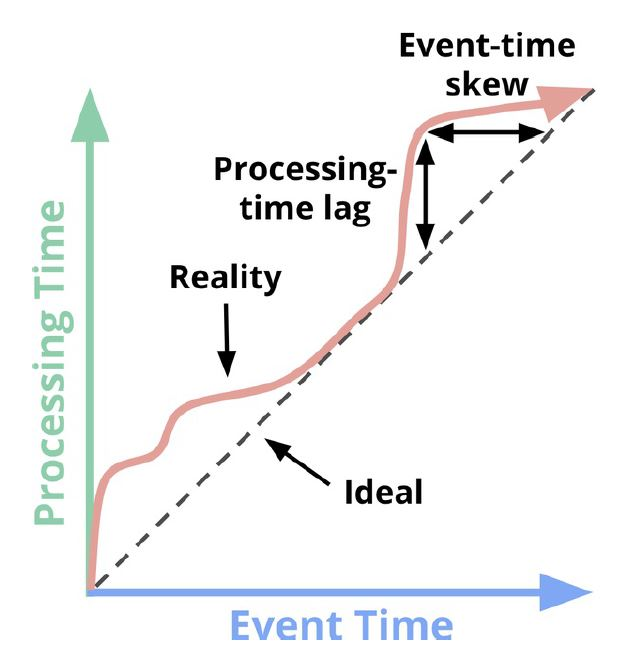
\includegraphics[scale=0.5]{1-processing-event-relationship}  
		\caption[Gambar Pemetaan {\it Time-Domain}]{Pemetaan {\it Time-Domain}} 
		\label{fig:processing-events relationship}
		\end{figure} 
		
		Sumbu X adalah \textit{event time} atau \textit{completeness} dalam sistem. Sumbu Y adalah 				\textit{Processing time} waktu jam biasa yang diamatai oleh sistem data processing ketika 				sedang dieksekusi. \textit{Processing-time lag} adalah jarak vertikal antara garis ideal 				dengan garis merah yang menunjukan ada berapa banyak waktu delay yang sedang diobservasi di 			antara kejadian pada waktu tertentu dan kapan delay itu terjadi. \textit{event-time skew} 				adalah garis horizontal dari garis ideal dengan garis merah yang menunjukan banyaknya 					distribusi data di \textit{pipeline} pada saat itu dan menunjukan seberapa ketinggalan suatu
		\textit{pipeline} dari \textit{pipeline} ideal.          

		\item \textbf{Studi literatur mengenai pola teknik pemrosesan \textit{stream processing}}\\
		{\bf Status :} Ada sejak rencana kerja skripsi.\\
		{\bf Hasil :} Pola-pola teknik pemrosesan \textit{stream procesing} dibagi menjadi dua yaitu
		\textit{batch} dan \textit{streaming}. Pola yang tergolong ke dalam \textit{batch} tidak 				dirancang untuk data yang tidak terbatas. Tetapi pemrosesan data tidak terbatas bisa 					dilakukan dengan membagi dataset menjadi beberapa bagian yang berisi potongan-potongan dari 			dataset tersebut yang lebih kecil dan terbatas. Sehingga bisa diproses dengan \textit{batch 			processing}. 
		Beberapa jenis \textit{batch processing} adalah \textit{fixed windows} dan \textit{Session}:
		\begin{itemize}
			\item{\textbf{\textit{fixed windows}} adalah pemrosesan paling umum. \textit{batch 						processing} ini bekerja dengan membagi input data ke beberapa \textit{windows} dan 						memproses \textit{window} tersebut secara terpisah. Proses ini dilakukan secara 						berulang-ulang. Jika data terkena delay gara-gara partisi \textit{network} perlu 						dilakukan mitigasi yang memperlambat proses yang memperlambat sampai semua data 						terkumpul.
			\begin{figure}[H] 
					\centering  
					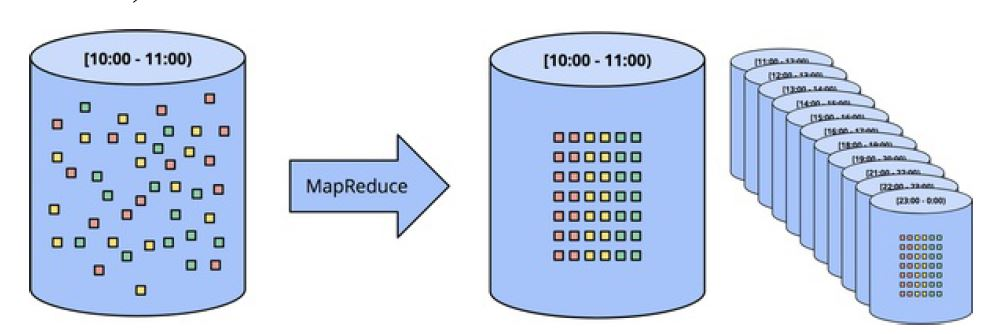
\includegraphics[scale=0.5]{3-fixed-windows}  
					\caption[Gambar {\it fixed-windowa}]{pemrosesan data tidak terbatas dengan 								menggunakan \textit{fixed window}} 
					\label{fig:processing-events relationship} 
					\end{figure} 			
			} 
			
			\item{\textit{Session} memiliki cara kerja yang hampir sama dengan \textit{fixed 						windows} bedanya pemotongan data dipisah berdasarkan session sehingga pembagian data 					jadi tidak seimbang data yang sama mungkin berakhir di \textit{batch} berbeda.}
		\end{itemize}
		
		Sedangkan pola-pola yang dikelompokan menjadi \textit{streaming} khusus dibangun untuk 					memproses data tidak terbatas. Karena pada dunia nyata banyak data yang tidak terstruktur
		dan tidak sekuensial. Sehingga jika suatu data ingin dianalisis dalam konteks data itu masih 		baru, harus ada sebuah metode pada \textit{pipeline} untuk mengurutkan data berdasarkan 				waktu ada 3 pola yang digunakan untuk \textit{stream processing} yaitu; \textit{filtering},
		\textit{approximation algorithm} dan \textit{windowing}.
		
		\begin{itemize}
			\item{\textit{\textbf{Filtering}} adalah operasi mendasar dan dilakukan secara \textit{Time-Agnostic} yang 
	memilah data yang masuk. Pola \textit{Time-Agonstic} digunakan untuk kasus-kasus dimana waktu 
	tidak relevan. Artinya, semua logika dan informasi pada data yang relevan ada pada data dan 
	yang lebih menentukan relevansi dari suatu data adalah urutan kedatangan data 
	tersebut. Jadi, pola ini hanya membutuhkan streaming engine yang mendukung pengiriman 
	data yang sederhana karena itu semua sistem streaming bisa menggunakan pola Time-
	AgnosticSistem melihat setiap rekord yang datang dan melihat apakah domain data 	
	sama dengan domain tujuan. Bila tidak data akan dibuang karena itu proses ini hanya 			
	bergantung pada urutan kedatangan data bukan dari \textit{event-time}.
	
	\begin{figure}[H] 
	\centering  
	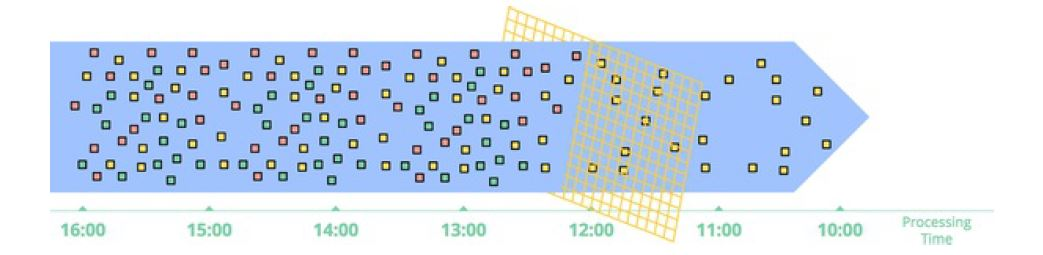
\includegraphics[scale=0.5]{8-Filtering-Unbounded-data}  
	\caption[Gambar {\it Filtering-unbounded-data}]{\textit{Filtering data}} 
	\label{fig:processing-events relationship} 
	\end{figure} 
	
	proses di atas adalah proses \textit{filtering data} dari kumpulan data yang
	heterogen menjadi homogen dengan tipe yang sama dan diletakan pada klaster yang sama.salah
	satu cara untuk mengelompokan data yang bersifat sama adalah dengan melakukan \textit{Inner 
	Join}.\textit{Inner Join} adalah salah satu bagian dari filtering dimana proses menggabungkan 
	dua sumber data yang tidak terbatas. Jika ada suatu data datang sistem akan menyimpan data 
	tersebut ke \textit{persistent state} ketika data berikutnya datang sistem akan 
	menggabungkan data tersebut dengan data yang ada di persistent state.
			}
			
			
			\item{\textbf{\textit{Approximation Algorithm}} adalah algoritma pendekatan yang 						menerima input data tidak terbatas dan mengelompokan data tersebut menjadi berdekatan 					jika memiliki sesuatu kesamaan. Konsep cara kerjanya hampir sama dengan 								\textit{clustering}. Tetapi \textit{approximation algorithm} merupakan algoritma 						yang rumit sehingga algoritma pendekatan susah untuk dipanggil ketika dibutuhkan dan 					proses pengelompokan dari algoritma ini cenderung terbatas.
			
			\begin{figure}[H] 
			\centering  
			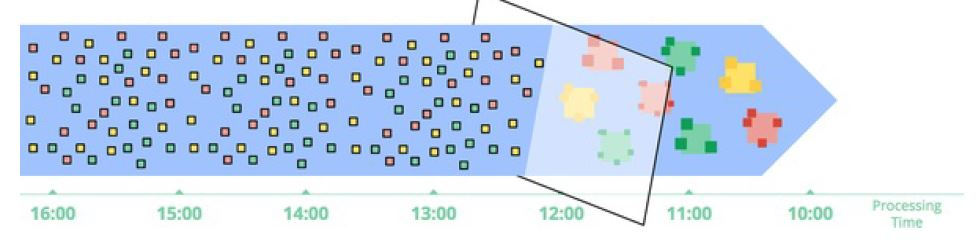
\includegraphics[scale=0.5]{5-approximation-algorithm}  
			\caption[Gambar {\it approximation-algorithm}]{Algoritma pendekatan pada 								\textit{unbounded data}} 
			\label{fig:processing-events relationship} 
			\end{figure} 
			
			Data dijalankan melewati algoritma yang kompleks dan menghasilkan data output yang 						terlihat lebih mirip hasil yang diinginkan. Algoritma pendekatan langsung memproses data 			yang datang karena itu melibatkan \textit{processing-time} digunakan algoritma sebagai 					pengecek \textit{error} pada data dengan membaca waktu urutan kedatangan dari data.
			}
			
			
			\item{\textbf{\textit{Windowing}} adalah fungsi yang menerima sumber data sebagai input.
			Lalu, membagi data tersebut menjadi beberapa bagian dan memberi batasan pada potongan 					data tersebut bisa dilihat pada gambar 4
			
				\begin{figure}[H] 
				\centering  
				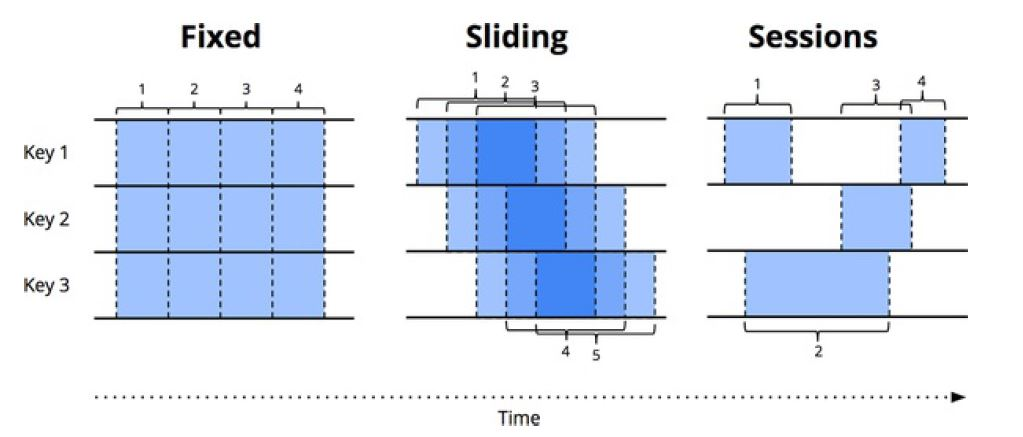
\includegraphics[scale=0.5]{7-Windowing}  
				\caption[Gambar {\it Windowing}]{Teknik Windowing} 
				\label{fig:processing-events relationship} 
				\end{figure}
				
			\textit{Fixed Windows} membagi waktu menjadi segmen-segmen dengan ukuran yang tetap. 					Seperti pada gambar 4. Segmen untuk fixed window diterapkan secara seragam pada seluruh 				dataset. Pembagian segmen dengan ukuran yang sama disebut aligned window. Tetapi, 						terkadang window tidak dibagi dengan ukuran yang sama. Dalam beberapa kasus, pembagian 					data bergantung pada ukuran dataset dan bervariasi tiap dataset. Pembagian waktu yang 					tidak merata, unaligned window, membantu 	meratakan penyebaran waktu penyelesaian.
			
			\textit{Sliding Windows} memiliki panjang dan periode yang tetap. Jika periode lebih 					kecil dari length maka terjadi overlap pada windows. Jika periode sama dengan waktu maka 			window akan menjadi fixed window. Jika periode lebih besar dari length maka akan menjadi 			sampling window yang hanya akan melihat suatu subset data dengan waktu yang lama.
			
			\textit{Dynamic Sessions} biasanya digunakan untuk menganalisa perilaku pengguna secara 				berkala dengan megelompokan suatu rantaian peristiwa yang berhubungan. contohnya adalah 				berapa banyak video yang ditonton oleh pengguna dalam sekali duduk. Panjang dari suatu 					sesi tidak bisa ditentukan terlebih dahulu. Panjang sesi tergantung dari seberapa banyak 			data yang terlibat. \textit{Dynamic Session} merupakan salah satu penerapan unaligned 
			window 	karena untuk setiap session subset pada suatu dataset tidak pernah identik.\\
			
			Selain itu Windowing bekerja dengan dua cara berbeda. Seperti \textit{Processing-time 
	Windowing} dimana Sistem menyimpan sementara data yang datang pada window untuk beberapa saat 
	sampai processing time telah lewat. Contohnya; misalkan ada fixed windows dengan durasi 5 			
	menit, sistem akan menyimpan sementara data selama lima menit waktu pemrosesan. Lalu, 			 
	sistem akan mengirim data yang telah diobservasi selama lima menit tersebut ke 				 
	\textit{downstream} untuk diproses.
	
	Proses windowing ini sangat simpel dan implementasinya mudah karena sistem tidak harus 		 
	mengatur data sesuai waktu. data hanya akan disimpan sementara ketika datang dan 				 
	langsung dilempar ke downstream ketika processing time selesai. Karena sistem bisa 			 
	mengetahui semua input karena telah dilihat oleh window. Sehingga sistem bisa dengan 			 
	baik memprediksi kapan suatu window akan selesai. metode yang kedua adalah \textit{Event-time 
	Windowing} Event-time Windowing digunakan ketika sistem mengobservasi sumber data yang tidak 
	terbatas dalam potongan-potongan data yang terbatas berdasarkan kapan data itu terjadi.
			}
		\end{itemize}\newpage
		
		

		\item \textbf{Studi literatur arsitektur \textit{Stream Processing}}\\
		{\bf Status :} Ada sejak rencana kerja skripsi.\\
		{\bf Hasil :}Arsitektur pada \textit{stream processing} dibagi menjadi dua Arsitektur lambda
		dan arsitektur kappa.\textbf{ Arsitektur Lambda} adalah teknik pemrosesan data yang bisa 				menangani data yang besar dengan cara mneggabungkan metode \textit{batch} dan \textit{stream 		processing}. Teknik ini menyeimbangkan antara \textit{latency, throuhput, dan fault-					tolerance} dengan menggunakan batch processing yang menyediakan penyimpanan data yang akurat 		dan komperhensif. Juga memanfaatkan stream processing agar mendapat data tidak terbatas 				secara \textit{realtime}.
		
		Banyak perusahaan yang menggunakan metode stream procesing untuk memprediksi updates dari 				model dan menyimpan event yang berbeda yang digunakan sebagai bahan untuk memprediksi. Untuk 		menangani kejadian seperti itu, Arsitektur Lambda memilki tiga layer; \textit{Batch layer}, 			\textit{speed layer (stream layer)}, dan \textit{Serving layer}.
		
		\begin{figure}[H] 
		\centering  
		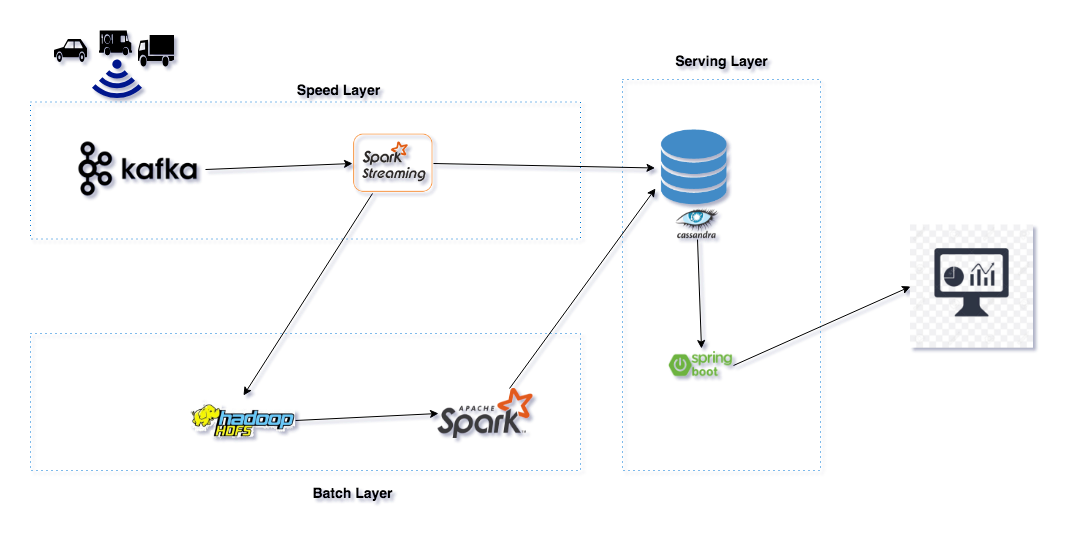
\includegraphics[scale=0.45]{lambda-architecture}  
		\caption[Gambar Arsitektur { \it Lambda}]{Arsitektur {\it Lambda}} 
		\label{fig:processing-events relationship} 
		\end{figure}
		
		\textit{batch layer} terlebih dahulu memproses data dengan menggunakan sistem 							terdistribusi yang bisa menangani data yang besar. tujuan dari batch layer adalah untuk 				meningkatkan akurasi dengan cara memproses semua data yang ada ketika membangun view. 					Artinya, batch layer bisa memperbaiki error pada data dengan memproses data kembali 					berdasarkan dataset yang sudah lengkap.
		
		Setiap data yang terus menerus datang ke sistem akan diteruskan ke batch layer dan stream 				layer secara bersamaan. Data Stream yang baru masuk ke batch layer langsung diproses pada 				data lake. Data disimpan pada data lake menggunakan in-memory database atau long term 					persistent database seperti NoSQL. Data akan diproses menggunakan MapReduce atau machine-				learning. Apache hadoop digunakan di layer ini karena memiliki throughput yang paling 					tinggi.
		
		\textit{Speed Layer(Stream Layer)} memproses data stream secara real-time tanpa 						 memperdulikan \textit{completeness} atau akurasi dari data. layer ini mengurangi 						\textit{throughput} untuk mengurangi \textit{latency}. Sehingga data yang terbaru bisa 					langsung dilihat. \textit{Speed layer} digunakan untuk mengisi jarak yang disebabkan oleh 				batch layer dengan memberikan informasi tentang data terkini. View yang dihasilkan dari 				layer ini belum tentu akurat namun bisa langsung dilihat dan diakses. Data yang lebih 					akurat akan disediakan dan diganti nanti oleh hasil data yang telah diolah oleh batch layer 			ketika sudah tersedia.
		
		\textit{Serving Layer} Output dari batch dan Speed layer diteruskan dan disimpan di layer 				ini dan proses \textit{ad-hoc queries} akan dilakukan di layer ini dengan mengembalikan 				views dari data yang telah diproses.
		
		Arsitektur Lambda dapat dianggap sebagai arsitektur pemrosesan data yang real-time. Seperti 			disebutkan di atas, dapat menahan kesalahan serta memungkinkan skalabilitas. Arsitektur ini 			menggunakan fungsi-fungsi batch dan stream lalu menambahkan data baru ke penyimpanan utama 				sambil memastikan bahwa data yang ada akan tetap utuh. Perusahaan seperti Twitter, Netflix, 			dan Yahoo menggunakan arsitektur ini untuk memenuhi kualitas standar layanan.
		
		
		Keuntungan dari Arsitektur Lambda antara lain adalah; \textit{Batch Layer} dari arsitektur 				ini mengatur histori data dengan penyimpanan terdistribusi yang \textit{fault tolerant} yang 		mana akan memperkecil terjadinya error walaupun sistem \textit{crash}, seimbang antara 					kecepatan dan keandalan, Scalable dan fault tolerant untuk data processing. Tetapi, 					arsitektur ini memiliki kelemahan yaitu; penerapan yang cukup sulit karena melibatkan 					\textit{batch} dan \textit{stream processing}, memproses setiap batch pada beberapa 					\textit{cycle} tidak menguntungkan untuk beberapa skenario, data yang dimodelkan dengan 				arsitektur ini susah untuk dimigrasi dan diorganisir ulang.
		
		\textbf{Arsitektur Kappa} simplifikasi dari arsitektur lambda. Susunan arsitektur ini hampir 		sama dengan sistem arsitektur lambda namumn tidak memiliki \textit{batch layer}. Untuk 					mengganti \textit{batch processing} data langsung diteruskan ke sistem streaming. Arsitektur 		ini digunakan model data berupa; beberapa \textit{event} atau \textit{query} data dicatat 				dalam suatu antrian untuk disesuaikan dengan penyimpanan atau riwayat sistem file 						terdistribusi, urutan \textit{event} dan \textit{query} tidak ditentukan sebelumnya, 					platform \textit{stream processing} dapat berinteraksi dengan basis data kapan saja. model 				ini sangat \textit{resilient} dan bisa menangani beberapa terabyte data untuk penyimpanan 				yang diperlukan untuk setiap sistem node yang mendukung replikasi.

		Skenario data yang disebutkan di atas ditangani oleh \textit{Apache kafka} yang cepat, 					toleran terhadap kesalahan dan dapat diskalakan secara horizontal. Hal ini memungkinkan 				mekanisme yang lebih baik untuk mengatur aliran data. kerena kontrol yang seimbang pada 				\textit{stream processing} dan database maka hal ini memungkinkan aplikasi untuk bekerja 				sesuai ekspektasi.Kafka menyimpan data yang diminta untuk jangka waktu yang lebih lama dan 				meayani \textit{queries} analog dengan menautkannya ke posisi yang sesuai dari log yang 				disimpan. Manfaat dari arsitektur ini adalah bisa mempertahankan sejumlah besar data untuk 				menyelesaikan \textit{queries}

		keuntungan dari arsitektur ini adalah dapat digunakan untuk mengembangkan sistem data yang 				merupakan yang tidak membutuhkan \textit{batch layer}, Pemrosesan ulang hanya diperlukan 				saat kode berubah dan dapat digunakan dengan memori tetap,Lebih sedikit sumber daya yang 				diperlukan karena pembelajaran mesin dilakukan secara \textit{real-time}. Tetapi, tidak 				adanya \textbf{batch layer} dapat mengakibatkan kesalahan selama pemrosesan data atau saat 				memperbarui database yang mengharuskan untuk ada pemrosesan ulang atau rekonsilisasi.\\

		\item{\textbf{Studi literatur mengenai sistem terdistribusi \textit{Hadoop}}\\
		{\bf Status :} Baru ditambahkan semester ini.\\
		{\bf Hasil :}\textit{Apache Hadoop} merupakan sebuah \textit{framework} yang bersifat 
		\textit{open-source} untuk menulis dan menjalankan aplikasi terdistribusi untuk mengolah 
		data dalam ukuran besar. Proyek Hadoop disusun dengan tujuan untuk mengatasi masalah 
		skalabitas pada \textit{nutch}, sebuah \textit{open-source crawler} dan mesin pencarian. 
		Hadoop merupakan bagian dari implementasi hasil riset google mengenai sistem file 
		terdistribusi dan komputasi pararel.

		Hadoop dapat berjalan di atas klaster mesin-mesin dengan kekuatan pemrosesan yang setara
		dengan komputer komersial maupun berjalan dengan layanan komputasi \textit{cloud}  yang
		dapat diakses dengan mudah oleh klien. Sistem terdistribusi Hadoop tidak perlu menggunakan
		mesin-mesin berspesifikasi tinggi, karena beban pemrosesan akan didistribusikan ke masing-				masing mesin di dalam klaster. Sistem tersebut dapat memudahkan pengguna ketika sistem
		diperlukan untuk pengolahan data dengan ukuran lebih besar, karena penambahaan ukuran data
		hanya memerlukan tambahan mesin ke dalam klaster dengan spesifikasi yang sama atau mendekati
 		mesin-mesin lain dalam klaster.

		Mesin-mesin dalam klaster dapat menjadi lebih ekonomis dibandingkan dengan menggunakan
		sebuah mesin dengan sepsifikasi yang lebih baik. Hal ini terkait dengan penambahan ukuran
		data yang akan diproses serta kerusakan perangkat keras yang mungkin terjadi. Hadoop dapat
		mengatasi kasus kerusakan tersebut tanpa ada kehilangan data, tetapi penggunaan sebuah mesin
		saja memiliki resiko kehilangan data saat ada kerusakan. selain itu, penggatian sebuah mesin
		yang rusak di dalam klaster akan memerlukan biaya yang lebih kecil dibanding menggani mesin
		dengan spesifikasi tinggi.

		Hadoop memerlukan pengolahaan data dengan ukuran yang sangat besar, Sehingga pemindahan data
		berukuran besar tersebut melalui jaringan akan memperlambat jalannya proses. Oleh karena
		itu, data tersebut diperkecil dengan membagi data tersebut menjadi blok-blok data dan
		mendistribusikannya ke masing-masing mesin dalam klaster. Kode aplikasi yang merupakan
		sebuah pekerjaan di lingkungan Hadoop dan berukuran lebih kecil dibandingkan dengan data
		akan didistribusikan ke dalam mesin-mesin klaster. Dengan demikian, pekerjaan pemrosesan
		data akan terjadi di setiap mesin di dalam klaster terhadap blok-blok data yang ada pada
		masing-masing mesin klaster.

		\textbf{Arsitektur Hadoop}\newline
		Sebuah klaster hadoop terdiri dari mesin-mesin yang saling terhubung. Klaster hadoop
		mempunyai arsitektur master/slave dengan sebuah mesin sebagai master node dan mesin-mesin
		lain sebagai slave node seperti yang ditunjukan pada gambar. Setiap node tersebut akan
		mempunyai komponen penyimpanan berupa HDFS dan komponen komputasi berupa MapReduce. Seperti
		yang ditunjukan pada gambar dapat dilihat bahwa HDFS dan MapReduce pada node mempunyai
	  	\textit{daemon} dan tugas yang berbeda dengan komponen HDFS dan MapReduce yang ada pada
	  	 slave node. Perbedaan tugas-tugas tersebut akan dijelaskan dibagaian.

		\begin{figure}[H] 
		\centering  
		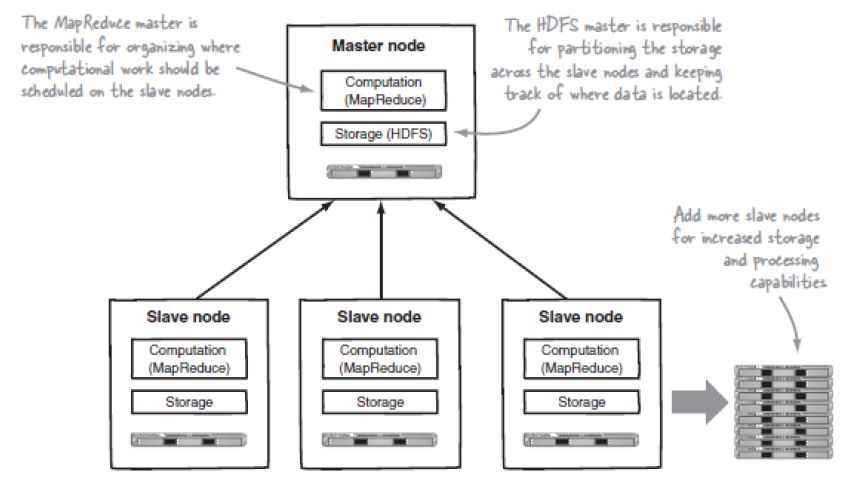
\includegraphics[scale=0.5]{Arsitektur-Hadoop}  
		\caption[Gambar Arsitektur { \it Hadoop}]{Arsitektur {\it Hadoop}} 
		\label{fig:processing-events relationship} 
		\end{figure}
		\begin{itemize}
		\item[]{\textbf{\textit{Hadoop Distributed File System}(HDFS)}\newline
		Hadoop distributed file system atau HDFS adalah komponen penyimpanan data dalam Hadoop.
		HDFS dirancang untuk memiliki \textit{throughput} tinggi dan cocok untuk melakukan 						operasi baca dan tulis pada file dengan ukuran yang sangat besar. Untuk mendukung hal 					tersebut, HDFS memanfaatkan ukuran blok data yang besar dan optimasi lokalitas data 					untuk mengurangi input output jaringan. Selain itu, data yang tersimpan di dalam HDFS 					tidak akan hilang ketika ada kerusakan pada salah satu mesin. Hal ini disebabkan adanya 				replikasi untuk setiap blok data yang terdistribusi di dalam klaster. Banyaknya 						replikasi yang terjadi pada awalnya adalah tiga, tetapi angka ini dapat dikonfigurasi 					ulang menjadi lebih sedikit maupun lebih banyak.
		
		\begin{figure}[H] 
		\centering  
		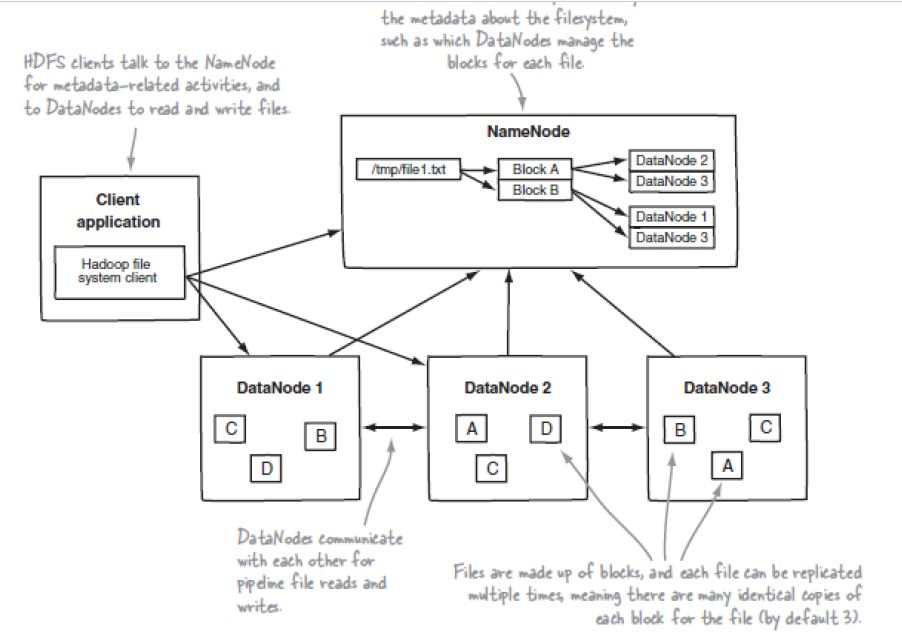
\includegraphics[scale=0.5]{HDFS}  
		\caption[Gambar Arsitektur { \it Hadoop}]{Arsitektur {\it HDFS}} 
		\label{fig:processing-events relationship} 
		\end{figure}
	
		Komponen HDFS pada master node menjalankan sebuah daemon yang disebut dengan NameNode. 					NameNode bertugas untuk mengatur pembagian blok-blok data ke slave node dan mencatat 					lokasi masing-masing blok data tersebut. NameNode Merupakan komponen yang penting dalam 				ekseskusi pemrosesan data dalam klaster. Berbeda dengan Master Node, komponen HDFS pada 				slave node menjalankan daemon yang disebut dengan DataNode. Data Node bertugas untuk 					melakukan proses baca tulis blok-blok data pada file asli yang terdapat sistem file 					lokal. Komunikasi pada awal operasi tulis atau baca terjadi diantara klien dan NameNode 				untuk mendapatkan lokasi blok-blok data yang akan diproses. setelah itu klien dapat 					berkomunikasi dengan DataNode lain untuk melakukan replikasi blok-blok data yang ada. 
	}
	
		\item[]{\textbf{\textit{MapReduce}}\newline
		MapReduce merupakan komponen komputasi dalam Hadoop. Model pemrograman yang dimiliki 					oleh MapReduce memungkinkan seorang programmer mengimplementasikan sebuah aplikasi yang 				berjalan paralel dengan mudah. Konfigurasi mengenai paralelisasi komputasi distribusi 					pekerjaan, dan cara mengatasi kegagalan perangkat lunak maupun keras telah ditangani
		oleh hadoop. Sehingga programmer hanya perlu mengimplementasikan pekerjaan pemrosesan 					apa saja yang perlu dilakukan.\newline
	
		\begin{figure}[H] 
		\centering  
		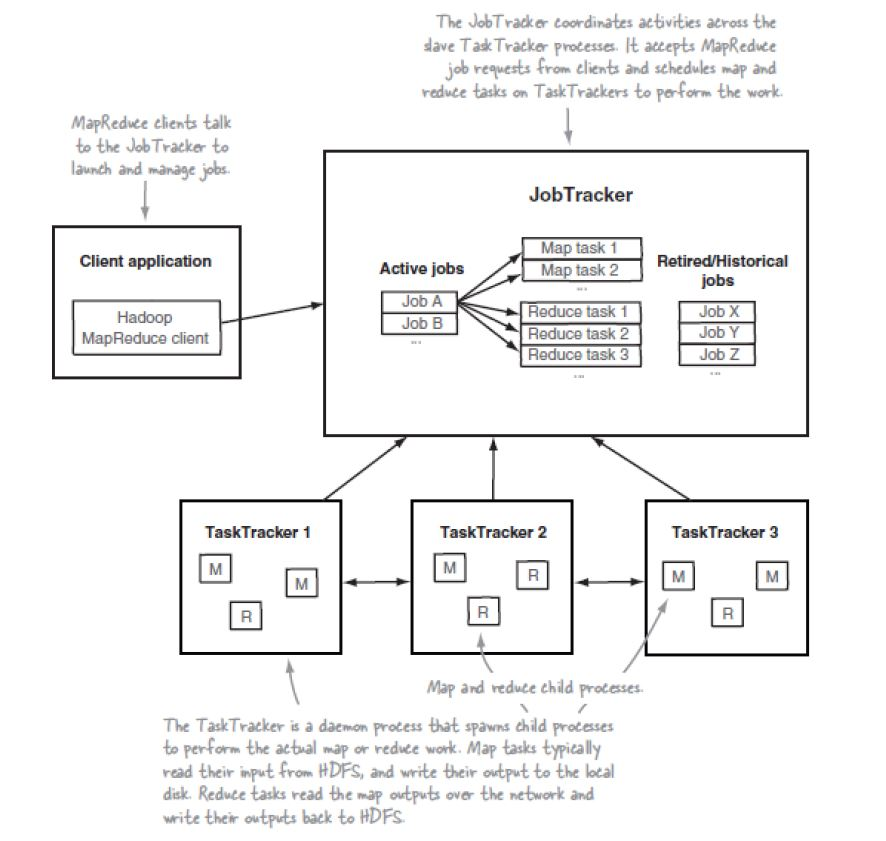
\includegraphics[scale=0.5]{Arsitektur-MapReduce}  
		\caption[Gambar Arsitektur Map Reduce]{Arsitektur Map Reduce} 
		\label{fig:processing-events relationship} 
		\end{figure}
	
		komponen MapReduce pada \textit{master node} menjalankan \textit{daemon} JobTracker 					yang merupakan \textit{daemon} JobTracker. MapReduce merupakan komponen komputasi dalam 				Hadoop. Model pemrograman yang dimiliki
		oleh MapReduce memungkinkan seorang programmer mengimplementasikan sebuah aplikasi yang
		berjalan paralel dengan mudah. Konfigurasi mengenai paralelisasi komputasi, distribusi 					pekerjaan, dan cara mengatasi kegagalan perangkat lunak maupun keras sudah ditangani oleh 				Hadoop, sehingga programmer hanya perlu mengimplementasikan pekerjaan pemrosesan apa saja 				yang perlu dilakukan
	
		\begin{figure}[H] 
		\centering  
		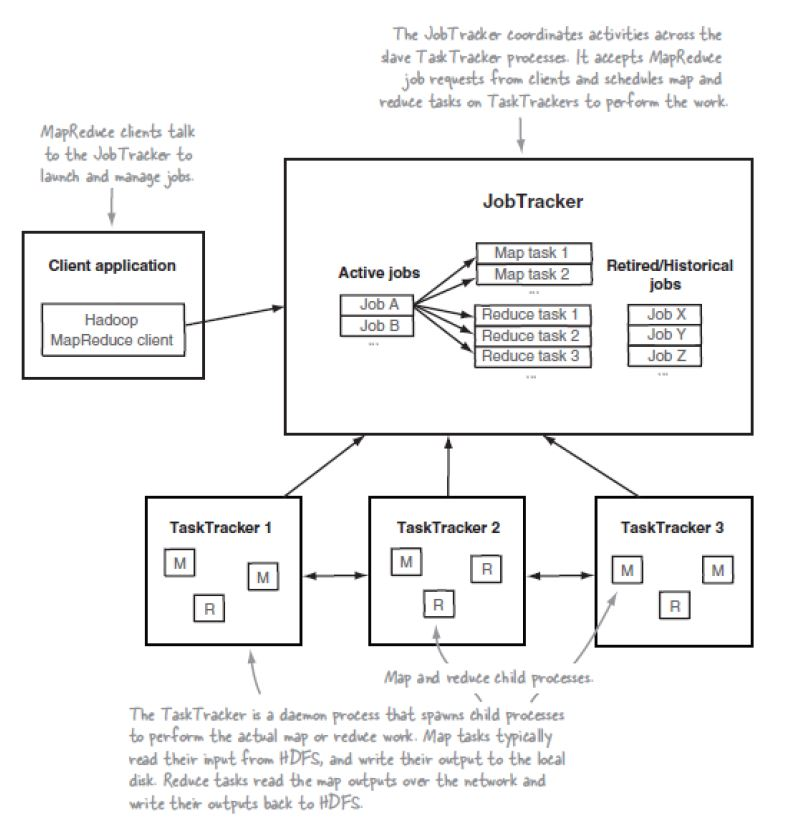
\includegraphics[scale=0.5]{mapreducearchitecture}  
		\caption[Gambar Arsitektur MapReduce]{Arsitektur MapReduce} 
		\label{fig:HDFS Architecture} 
		\end{figure}
		\newpage
		Komponen MapReduce pada master node menjalankan daemon JobTracker yang merupakan
		daemon yang menghubungkan proses pada Hadoop dengan aplikasi. JobTracker bertugas melakukan
		pemecahan pekerjaan yang dikirimkan klien menjadi unit-unit pekerjaan map dan reduce. Job-
		Tracker akan mendistribusikan unit-unit pekerjaan tersebut ke slave node, melakukan 					penjadwalan komputasi, dan melakukan pengawasan terhadap pemrosesan yang dilakukan dalam 				slave node.
		Komponen MapReduce pada setiap slave node menjalankan daemon TaskTracker yang bertugas
		untuk melakukan eksekusi pemrosesan di dalam slave node. TaskTracker akan selalu 						berkomunikasi
		dengan JobTracker untuk memantau jalannya proses. Jika komunikasi tersebut terputus, dapat
		diasumsikan proses pada TaskTracker tersebut gagal dan unit pekerjaan yang sesuai akan 					dikirimkan oleh JobTracker ke slave node lain yang terdapat di dalam klaster.
		MapReduce terdiri dari komponen-komponen mapper dan reducer. Pekerjaan yang dikirimkan
		ke dalam klaster akan dipecah menjadi pekerjaan map dan reduce yang berjalan secara paralel.
		Setiap node dalam map dan reduce dapat berdiri sendiri dan tidak tergantung pada node-node 				map atau reduce lainnya. Ketergantungan yang ada hanya ketergantungan node-node reduce 					terhadap
		node-node map. Pemrosesan ini dilakukan dengan model share-nothing, yaitu data yang diolah
		tidak dibagikan antarnode untuk mencegah node-node tersebut saling menunggu untuk memakai
		sumber daya. Implementasi aplikasi dengan MapReduce dapat dilakukan dengan mendefinisikan 				fungsi 	map dan reduce. Fungsi map menerima masukan berupa pasangan-pasangan key dan value 				dan memberikan keluaran berupa list key dan value. Fungsi reduce menerima masukan berupa key 		dan list value dan memberikan keluaran berupa pasangan key dan value.
	
		\begin{figure}[H] 
		\centering  
		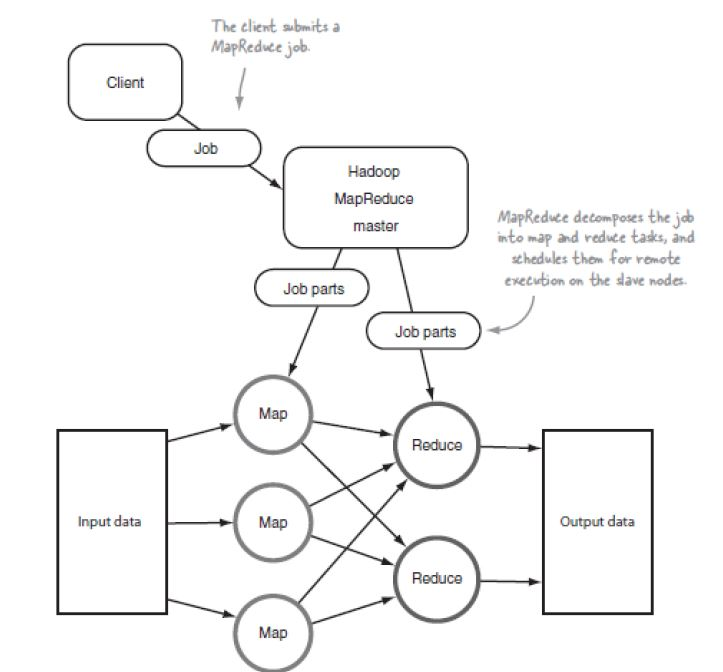
\includegraphics[scale=0.5]{MapReduceProses}  
		\caption[Gambar Proses MapReduce]{Proses MapReduce} 
		\label{fig:processing-events relationship} 
		\end{figure}
	
		Gambar merupakan gambaran proses yang terjadi ketika klien mengirimkan sebuah pekerjaan
		MapReduce ke dalam klaster. Pekerjaan yang dikirimkan oleh klien dapat berupa file jar atau
		xml. Pekerjaan tersebut akan dipecah menjadi unit-unit pekerjaan map dan reduce oleh 					komponen
		MapReduce yang terdapat pada master node sebelum didistribusikan ke slave node.
		Data masukan akan diproses menggunakan komponen mapper pada MapReduce dan format
		data harus berupa pasangan key dan value. Untuk setiap pasang key dan value tersebut, 					dilakukan
		pemrosesan menggunakan fungsi map dan mengembalikan keluaran berupa list pasangan key dan
		value yang baru. Nilai key pada tahap pemrosesan ini pada umumnya tidak diperhitungkan.
		Hasil keluaran dari mapper akan diproses terlebih dahulu sebelum dijadikan masukan untuk
		komponen reducer. Tahap pemrosesan ini disebut sebagai tahap shuffle and sort. Setiap 					pasangan
		key dan value akan diurutkan berdasarkan key yang dimiliki dan mengelompokkan semua value 				yang
		mempunyai key yang sama untuk dimasukkan ke node reducer yang sama. Proses ini akan menjadi
		kompleks ketika semua key yang ada dalam list keluaran mempunyai nilai yang berbeda-beda.
		Komponen reducer menerima masukan yang berasal dari hasil pada tahap shuffle and sort yang
		berupa pasangan key dan list value. Untuk setiap nilai key yang ada, fungsi reduce pada 				reducer
		akan dipanggil satu kali dan memberikan keluaran berupa pasangan key dan value yang baru.
		Keluaran dari proses reduce tersebut dapat ditulis ke file yang berada di HDFS maupun ke 				dalam basis data.
	
	}
\end{itemize}
		}
		
		\item{\textbf{Studi literatur mengenai sistem terdistribusi \textit{Spark}}\\
		{\bf Status :} Ada sejak rencana kerja skripsi.\\
		{\bf Hasil :}\textit{Apache Spark} merupakan \textit{platform} komputasi klaster yang 					dirancang untuk berjalan dengan cepat ketika mengolah data yang sangat besar dan untuk 					tujuan penggunaan umum. \textit{Spark} merupakan penerus dari model pemprosesan 						\textit{MapReduce} pada \textit{Hadoop} dengan jenis komputasi lebih banyak yang dapat 					dilakukan. Salah satu fitur utama yang ditawarkan \textit{Spark} untuk kecepatan adalah 				kemampuan untuk menjalankan komputasi di memori. Namun, sistem ini lebih efisien dari 					\textit{Map Reduce} untuk aplikasi kompleks yang berjalan pada disk karena \textit{Spark} 				menggunakan DAG(\textit{Directed Acyclic Graph}) \textit{Engine} yang mengoptimasi workflow. 		DAG bekerja dengan cara  menentukan jenis suatu flow yang akan memproses data yang masuk. 				\textit{Spark} akan mencari cara pengerjaan mana yang paling optimal untuk melakukan 					pendekatan bagi masalah ini secara keseluruhan. \textit{Spark} juga akan mengoptimasi 					\textit{workflow} dari pengerjaan tersebut. \textit{Spark} lebih bisa beradaptasi dengan 				pengerjaan pemrosesan data secara menyeluruh karena itu spark bisa bekerja dengan cepat.

		\textit{Spark} telah dioptimalkan untuk berjalan pada memori sehingga mempercepat 						pengolahaan data dibandingkan dengan pendekatan alternatif lain seperti \textit{Map Reduce} 			pada hadoop yang menulis dan membaca data secara langsung pada \textit{hard drive} komputer 			pada setiap tahap pemrosesan. Dengan demikian kecepatan pengolahaan data menggunakan spark 				dapat menjadi lebih cepat dibandingkan dengan Hadoop. 

		\textit{Spark} sering digunakan dalam pemanggilan kueri interaktif pada set data yang besar, 		pengolahaan data streaming dari sensor maupun sistem finansial, dan tugas-tugas pembelajaran 		mesin. Selain itu, pengembangan juga dapat menggunakan spark untuk tugas-tuga pemrosesan 				data lainnya dengan memanfaatkan \textit{library} pengembang dan API serta dukungan untuk 				bahasa pemrograman java, Python, R, dan Scala. Spark biasa digunakan bersama dengan 					HDFS(\textit{Hadoop distributed File System}) sebagai pengganti media penyimpanan. 						\textit{Spark} mempunyai lima buah fitur kunci, yaitu; \textit{easy to use, fast, general 				purpose, scalable}, dan \textit{falut tolerant}.
		
		\begin{enumerate}
			\item{\textit{Easy to Use}: Spark menyediakan lebih dari 80 jenis operator untuk 						melakukan proses pengolahan data. Sehingga pengolahaan data yang lebih kompleks bisa 					dilakukan dengan mudah.}
	
			\item{\textit{Fast}:\textit{Spark} meminimalisir akses data pada disk dengan menyimpan 					data pada \textit{cache}. Sehingga pengolahaan data menggunakan set data yang sama hanya 			memerlukan akses pada disk sebanyak satu kali.}
	
			\item{\textit{General Purpose}: \textit{Spark} sudah mempunyai \textit{library} sendiri 				untuk melakukan \textit{batch processing}, analisis interaktif pada pengolahan 							\textit{data stream}, pembelajaran mesin dan komputasi graf. Setiap mesin tersebut tidak 			memerlukan mesin klaster tersendiri untuk melakukan jenis pengolahan tertentu sehingga 					mengurangi kompleksitas operasional dan menghindari duplikasi kode maupun data.}
	
			\item{\textit{Scalability}: Sama seperti pada Hadoop, peningkatan kapasitas pengolahan 					data dapat dilakukan dengan menambahkan mesin ke dalam klaster. Selain itu, penambahan 					mesin pada Spark memengaruhi kode aplikasi yang sudah ada.}
	
			\item{\textit{Fault Tolerant}: Kerusakan pada salah satu mesin pada klaster sudah 						ditangani oleh spark. Tetapi, perlu ada kode untuk menangani hal tersebut walaupun 						kerusakan tersebut tidak memengaruhi kinerja aplikasi.}
	
		\end{enumerate}	
		
		Sebuah proyek Spark mempunyai beberapa komponen yang terintegrasi dalam Spark Pada intinya, 			Spark adalah sebuah mesin komputasi yang bertugas untuk mendistribusikan dan memantau 					aplikasi yang terdiri dari banyak tugas komputasi yang tersebar  ke mesin pekerja atau 					klaster komputasi. Mesin inti Spark yang dapat berjalan cepat dengan tujuan penggunaan umum 			memberikan kekuatan tambahan untuk komponen dengan tingkatan yang tingkatan pada susunan 				yang dikhususkan untuk beban kerja yang beragam. Komponen-komponen ini dirancang untuk 					beroperasi dengan erat dan dapat digunakan dengan memanggil komponen ini sebagai library di 			dalam sebuah proyek perangkat lunak.

		\begin{figure}[H] 
		\centering  
		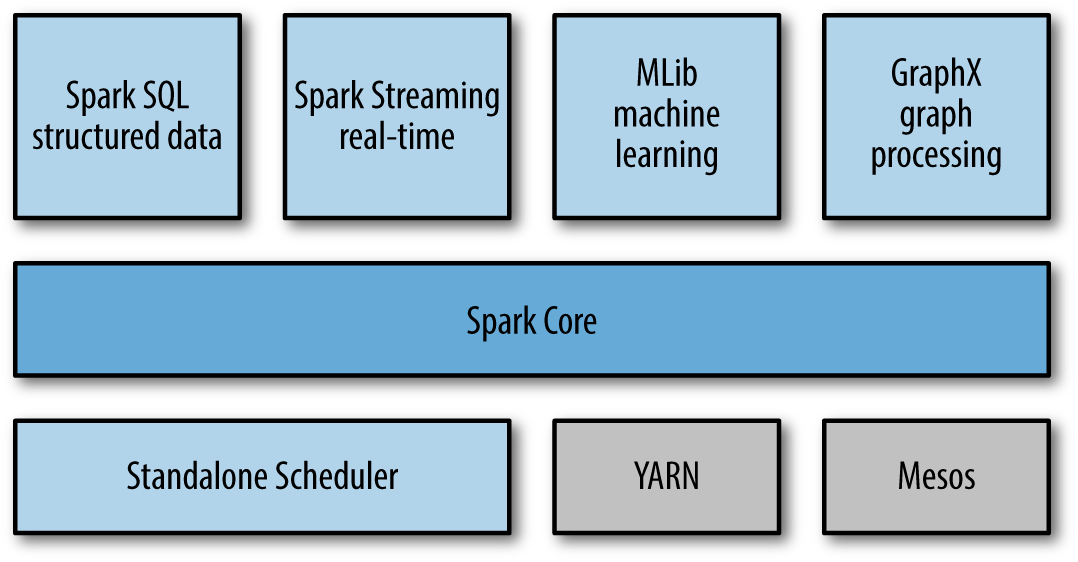
\includegraphics[scale=1]{spark-core}  
		\caption[Gambar { \it Spark unified stack}]{{\it Susunan Spark}} 
		\label{fig:processing-events relationship} 
		\end{figure}	
		
		}
		
	\begin{itemize}
		\item{\textit{Spark Core} \textit{Spark Core} merupakan fungsi dasar dari \textit{Spark} 				dan mempunyai komponen-komponen untuk penjadwalan tugas, pengelolaan memori, pemulihan 					kegagalan, berinteraksi dengan sistem penyimpanan, dan lainnya. \textit{Spark Core} juga 				mempunyai API untuk mendefinisikan \textit{Resilient Distributed Dataset}(RDD) serta 					\textit{Spark Context}.}
	
		\item{\textit{Spark SQL} Modul yang bekerja dengan data terstruktur menggunakan Hive yang 				memungkinkan programmer untuk menggabungkan SQL dengan bahasa pemrogramman spark seperti 				\textit{python, scala, dan 	java}.}
	
		\item{\textit{Spark Streaming} API yang menyediakan pemrosesan data secara \textit{real-				time}.komponen-komponen dari \textit{Spark Streming} hampir sama dengan \textit{Spark Core}. 		Seperti pengeloaan memori, pemulihan kegagalan, dan skalabilitas. \textit{Spark Streaming} 				mempunyai abstraksi dan API berupa \textit{Dstream} dan \textit{Streaming Context}. Spark 				Streaming akan dibahas lanjut pada 2.4.3}
	
		\item{\textit{Mlib} Sebuah \textit{library} untuk \textit{machine learning}yang menyediakan 			beberapa tipe algoritma pembelajaran mesin yang dirancang untuk bekerja lintas klaster.}
	
		\item API untuk pemrosesan \textit{graph} dan komputasi \textit{graph-parallel}.
	
		\item{\textit{Cluster Manager} Spark Dirancang untuk tetap efisien dalam peningkatan mesin 				dari satu hingga ribuan mesin. Untuk mencapai efisiensi tersebut sekaligus memaksimalkan 				fleksibilitas. Spark dapat menjalankan \textit{cluster manager} termasuk Hadoop dan YARN, 				Apache Mesos, dan 	\textit{Cluster Manager} yang sudah termasuk dalam spark yaitu 						Standalone Scheduler.}
	\end{itemize}
	
	\textit{\textbf{Application Programming Interface (API) Spark}} adalah Kemampuan komputasi pada 		aplikasi spark ada dalam bentuk \textit{library}. \textit{library} tersebut ditulis dalam bahasa 	scala. 	Tetapi, menyediakan \textit{Applicataion Programming Interface} atau API dalam berbagai 		bahasa. Spark API mempunyai dua abstraksi penting, yaitu \textit{Spark Context} dan 					\textit{Resilient Distributed Datasets}(RDD). Kedua Abstraksi ini memungkinkan sebuah aplikasi 			untuk berinteraksi dengan Spark, terhubung dengan klaster, dan menggunakan sumber daya dalam 			\textit{Cluster}.
	
	\textbf{Spark Context}\newline
	\textit{Spark Context} Merupakan sebuah kelas yang didefinisikan dalam \textit{library Spark}. 			Spark Context merepresentasikan sebuah koneksi ke cluster spark dan diperlukan untuk membuat 			objek-objek lain yang disediakan oleh \textit{Spark} API. Sebuah aplikasi harus mempunyai objek 		\textit{Spark Context} yang aktif. Objek \textit{Spark Context} tersebut harus mempunyai 				konfigurasi untuk alamat spark master dan nama aplikasi. Spark Master merupakan cara 					SparkContext terkoneksi dengan klaster. Penggunaan kata kunci lokal menjalankan Spark dengan 			menggunakan sebuah thread pada satu mesin saja. Penggunaan thread tersebut dapat dikonfigurasi 			menjadi local$[n]$ untuk n buah thread atau local$[*]$ untuk menggunakan thread sejumlah core.
	
	\textbf{Resilient Distributed Dataset(RDD)}\newline
	RDD adalah abstraksi dasar untuk merepresentasikan kumpulan objek yang dapat didistribusikan 			pada mesin-mesin dalam sebuah klaster. RDD dapat dibuat dengan menggunakan data yang bersumber 			dari luar seperti file dalam HDFS, tabel basis data, atau kumpulan objek local dan hasil 				transformasi yang dilakukan pada RDD yang sudah ada. Pembuatan RDD dengan data dari sumber luar 		memerlukan objek \textit{spark context}. karakteristik RDD.
	
	\begin{enumerate}
	\item{\textit{Immutable}\newline
	RDD merupakan sebuah struktur data yang permanen. RDD yang dibuat tidak dapat dimodifikasi lebih 	lanjut. Sehingga operasi yang mengubah RDD akan mengembalikan RDD yang baru.
	}
	
	\item{\textit{Partitioned}\newline
	Data yang direpresentasikan oleh RDD terbagi menjadi partisi-partisi yang didistribusikan pada 			klaster mesin-mesin. Akan tetapi, partisi-partisi tersebut akan berada pada sebuah mesin yang 			sama jika \textit{Spark} hanya berjalan pada satu mesin saja. Di antara partisi RDD dengan 				partisi fisik set data terdapat pemetaan. Jenis Pemetaan tergantung pada sumber data seperti, 			blok-blok data HDFS mempunyai pemetaan satu ke satu dengan partisi-partisi RDD dan berapa 				partisi-partisi RDD dan beberapa partisi \textit{cassandra} dipetakan ke satu buah partisi RDD.
	}
	
	\item{\textit{Fault Tolerant}\newline
	RDD mengatasi kegagalan dari mesin klaster secara otomatis. Partisi RDD yang hilang pada mesin 			yang rusak tersebut akan dibuat ulang pada mesin lain. Hal ini dapat dilakukan karena spark 			menyimpan informasi keterhubungan antara RDD dan informasi tersebut digunakan untuk memulihkan 			bagian atau keseluruhan RDD yang hilang.
	}
	
	\item{\textit{Interface}\newline
	RDD merupakan sebuah antar muka untuk pemrosesan data yang didefinisikan sebagai kelas 					abstrak dalam \textit{library Spark}. RDD menyediakan antarmuka yang seragam untuk 						pemrosesan data yang berasal dari berbagai sumber. Selain itu RDD juga menyediakan kelas-				kelas implementasi konkret untuk sumber data yang berbeda.	
	}
	
	\item{\textit{Strongly typed}\newline
	Definisi kelas RDD mempunyai parameter tipe yang memungkinkan RDD untuk 								merepresentasikan data dengan tipe berbeda. RDD merupakan kumpulan elemen homogen yang 					terdistribusi dan elemen-elemen tersebut dapat bertipe \textit{Integer, Long, Float, 					String}, atau tipe yang didefinisikan oleh pengembang aplikasi.
	}
	
	\item{\textit{In Memory}\newline
	Kelas RDD menyediakan API untuk komputasi klaster dalam memori. \textit{Spark} 							memungkinkan RDD untuk di-cache atau dipertahankan dalam memori. Operasi pada RDD yang 					ada dalam cache berjalan lebih cepat dibandingkan dengan operasi pada RDD yang tidak 					berada dalam cache.
	}
\end{enumerate}

Data yang sudah direpresentasikan dalam RDD dapat dioperasikan dengan menggunakan dua jenis operasi dasar, yaitu transformasi dan aksi.
\begin{enumerate}
	\item{\textit{transformasi}\newline
	RDD yang menjadi masukan dari sebuah operasi transformasi akan mengalami perubahan struktur 			atau nilai yang ada pada RDD. karena RDD bersifat \textit{immutable}, maka perubahan dari 				operasi ini secara konseptual akan dikembalikan dalam bentuk RDD baru.
	}
	
	\item{\textit{Aksi}\newline
	Operasi menjadi titik awal dari komputasi-komputasi yang telah terjadi pada RDD masukan. 				Pemanggilan operasi aksi akan memulai pembentukan RDD yang diperlakukan untuk komputasi. 				Operasi ini menerima masukan berupa RDD dan meberikan hasil berupa sebuah nilai.
	}
\end{enumerate}

Operasi yang dilakukan pada RDD bersifat \textit{lazy} yang berarti operasi tersebut tidak akan dieksekusi oleh spark sampai ada operasi aksi. Evaluasi \textit{lazy} berarti ketika ada pemanggilan operasi transformasi pada RDD. Operasi tersebut tidak langsung dilakukan spark mencatat metadata untuk menandakan bahwa operasi tersebut sudah pernah diminta. Dengan demikian, RDD dapat disebut sebagai kumpulan instruksi untuk melakukan komputasi data yang dibuat dari kumpulan operasi transformasi.

		\item \textbf{Studi Literatur Spark: Arsitektur Spark}\\
		{\bf Status :} Ada sejak rencana kerja skripsi\\
		{\bf Hasil :} \newline
			\begin{figure}[H] 
			\centering  
			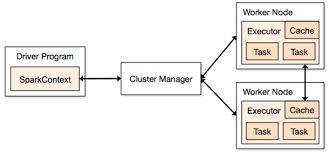
\includegraphics[scale=0.8]{spark-arsitektur}  
			\caption[Gambar Arsitektur {\it Spark}]{Arsitektur {\it Spark}} 
			\label{fig:processing-events relationship} 
			\end{figure}
	
		Berdasarkan pada gambar sebuah aplikasi melibatkan lima entitas penting yaitu; driver 					program, cluster manager, worker, executor, dan task.
		
	\begin{enumerate}
	\item{\textit{Driver Program}\newline
	Driver Program merupakan bagian dari aplikasi yang memulai menjalankan proses pengolahan 				data yang akan dilakukan. Driver program terhubung dengan komponen-komponen lain melalui 				objek \textit{Spark Context} yang terdapat dalam komponen ini. Objek \textit{Spark Context}
	akan melakukan koneksi dengan \textit{cluster manager}. Setiap klaster hanya akan mempunyai 			satu buah driver program atau satu buah objek spark context. 
	}
	
	\item{\textit{Cluster Manager}\newline
	\textit{Cluster Manager} berfungsi untuk mengelola sumber daya yang digunakan untuk proses 				pengolahan. Spark Context pada komponen driver program dapat terhubung dengan salah satu dari 			jenis-jenis cluster manager yang didukung oleh Spark, yaitu \textit{cluster manager} seperti 			\textit{Apache mesos} dan \textit{Yarn}. Setiap Cluster hanya memiliki satu buah 						\textit{cluster manager}.
	
	\item{\textit{Worker}\newline
	Worker merupakan komponen yang menyediakan unit pemrosesan dan alokasi memori untuk 					menyimpan sumber daya yang digunakan dalam proses yang berjalan. Setiap klaster dapat 					memiliki lebih dari satu buah worker dan setiap worker tersebut akan menjalankan aplikasi 				sebagai proses yang terdistribusi pada sebuah klaster.
	}
	
	\item{\textit{Executor}\newline
	\textit{Executor} merupakan proses yang dibuat oleh \textit{spark} pada setiap node worker 				untuk menjalankan aplikasi. \textit{Executor} yang terdapat pada setiap worker hanya dapat 				menangani proses untuk sebuah aplikasi saja, sehingga aplikasi yang berbeda akan mempunyai 				eksekutor yang berbeda. Setiap eksekutor mempunyai lama hidup yang sama dengan aplikasi 				sehingga akan berhenti ketiak aplikasi berhenti berjalan. Setiap Klaster dapat mempunyai 				lebih dari satu eksekutor dan jumlah tergantung pada banyak aplikasi.
	}
	
	\item{\textit{Task}\newline
	\textit{Task} merupakan unit pekerjaan terkecil yang dikirimkan ke executor. Unit pekerjaan 			tersebut akan dijalankan pada sejumlah \textit{thread} yang terdapat pada executor. Banyak 
	\textit{Thread} yang digunakan berbanding lurus dengan banyak partisi data yang diolah.
	}
		
	}
\end{enumerate}

		\item \textbf{Studi literatur mengenai \textit{Spark Streaming}} \\
		{\bf Status :} Ada sejak rencana kerja skripsi.\\
		{\bf Hasil :}\textit{Spark Streaming} adalah ekstensi dari API \textit{Spark Core} yang 				menyediakan pemprosesan \textit{Data Stream} yang bisa ditingkatkan performanya dengan 					menambah \textit{hardware baru}, bisa memproses data dengan banyak dan cepat, dan sistem 				masih bisa beroperasi ketika terjadi kegagalan. Data bisa dikumpulkan dari berbagai sumber 				seperti \textit{Kafka, Flume, Kinesis, atau TCP Socket}. Data yang terkumpul akan langsung 				diproses dengan algoritma yang kompleks seperti \textit{Map, Reduce, Join} dan 							\textit{Windowing}. Terakhir data yang telah diproses langsung dikirim ke \textit{File 					Systems, database} dan \textit{live dashboard}. Penjelasan lebih jelas ada pada gambar 2.12 			berikut:

		\begin{figure}[H] 
		\centering  
		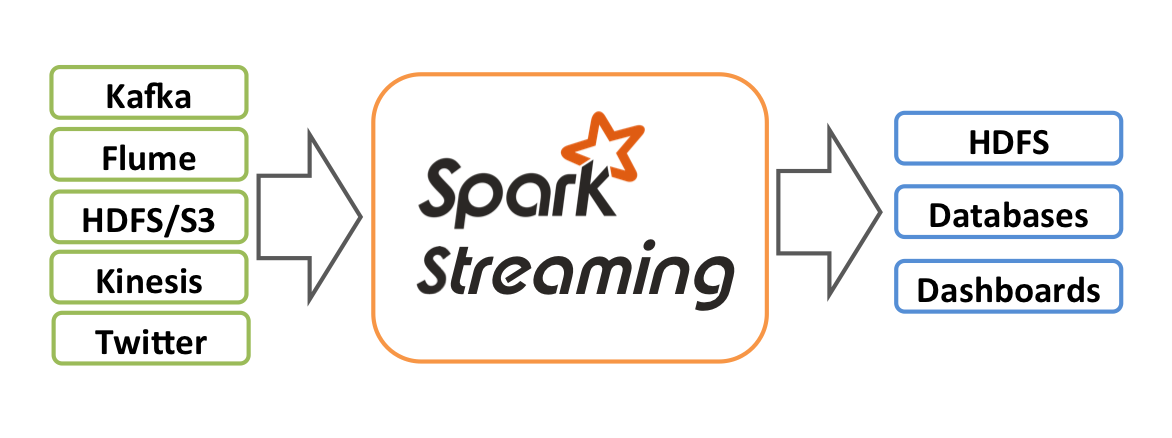
\includegraphics[scale=0.7]{streaming-arch}  
		\caption[Gambar Arsitektur {\it Spark Streaming}]{Arsitektur {\it Spark Streaming}} 
		\label{fig:processing-events relationship} 
		\end{figure}
		
		\textbf{Arsitektur \textit{Spark Streaming}}
		\textit{Spark Streaming} bekerja dengan cara menerima input \textit{data streams}secara 				langsung dan membagai data tersebut menjadi beberapa potongan-potongan(\textit{batches}), 				yang nanti akan diproses oleh mesin \textit{Spark} untuk menghasilkan \textit{stream} akhir 			pada \textit{batches}. \textit{Spark Streaming} tidak memproses data secara periodik, hanya 			memproses yang duluan datang dan memutakhirkan hasil dari \textit{Spark Streaming} dari 				waktu ke waktu. Data langsung bisa dianalisis ketika datang dengan mengelompokannya ke 					beberapa bagian kecil dan langsung melakukan agregasi pada potongan data tersebut.
		
		\begin{figure}[H] 
		\centering  
		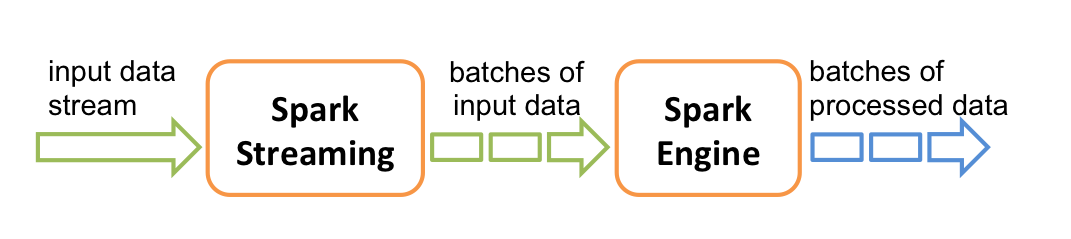
\includegraphics[scale=0.7]{streaming-flow}  
		\caption[Gambar Arsitektur {\it Spark Streaming}]{Arsitektur {\it Spark Streaming}} 
		\label{fig:processing-events relationship} 
		\end{figure}
	
	
		Berdasarkan gambar 2.13 \textit{Data Streams} yang masuk akan diterima oleh 							\textit{reciever} lalu potongan-potongan data yang masuk pada selang waktu tertentu akan 				dihasilkan secara terus menerus dengan kata lain proses transformasi akan terus berlangsung 			ketika program dihentikan.Lalu, data yang telah dihasilkan dapat dikirimkan langsung ke 				\textit{external database} dengan data yang telah diagregasi sebelumnya.

		transformasi dan aksi pada RDD bisa terjadi secara pararel pada node \textit{worker}. 					Artinya, proses RDD dibagi menjadi potongan kecil dan didistribusikan, potongan yang berbeda 		akan dikirim ke node yang berbeda. Potongan RDD tersebut akan didistribusikan ke seluruh 				klaster.

		Aplikasi \textit{Spark Streaming} membutuhkan pengaturan tambahan untuk beroperasi tanpa 				henti. Aturan yang dimaksud adalah \textit{checkpointing} yang merupakan mekanisme utama 				pada \textit{Spark Streaming}. \textit{Checkpointing} memungkinkan penyimpanan data pada 				\textit{file system} seperti HDFS dan yang membuat \textit{Spark Streaming} menjadi 					\textit{fault tolerant}.
		
		\textbf{Abstraksi \textit{Spark Streaming}}\newline
		
		Abstraksi dasar yang disediakan oleh \textit{Spark Streaming} disebut \textit{Discretized 				Streams} (\textit{DStreams}). \textit{Dstream} merupakan seluruh alur data yang datang dari 			\textit{recievers} Setiap Dstream dibuat pada potonga-potongan RDD yang merepresentasikan 				aliran data yang kontinu. Dstream memiliki dua buah operasi; transformasi dan \textit{output 		operation}. Transformasi bertugas untuk menghasilkan Dstream baru dan \textit{Output 					operation} bertugas untuk menuliskan data ke sistem eksternal. \textit{Dstream} menyediakan 			operasi yang hampir sama dengan operasi RDD dan mempunyai operasi sendiri yang digunakan 				untuk mengatur waktu seperti \textit{sliding window}.
 
		setiap RDD yang ada pada Dstream mempunyai data dari interval tertentu yang akan ditunjukan 			pada gambar 2.14

		\begin{figure}[H] 
		\centering  
		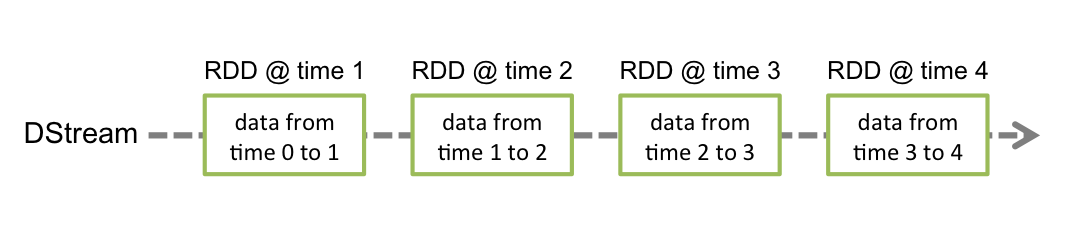
\includegraphics[scale=0.7]{streaming-dstream}  
		\caption[Gambar Alur {\it Dstream}]{Alur {\it Dstream}} 
		\label{fig:processing-events relationship} 
		\end{figure}

		Pada setiap awal interval, \textit{batch} baru selalu dibuat dan setiap data yang muncul 				pada interval tersebut akan dimasukan ke \textit{batch} tersebut. Saat interval berakhir 				\textit{batch} telah selesai berkembang. Ukuran dari suatu interval ditentukan oleh sebuah 				parameter yang disebut \textit{batch interval}. Biasanya, ukurandari interval berkisar 					antara 500 milidetik sampai beberapa detik. Setiap input yang ada di dalam batch membentuk 				RDD dan diproses menggunakan \textit{Spark Jobs} untuk membuat RDD lain. RDD akan terus 				dibuat dan ditransformasi terus menerus sampai ada aksi yang memberhentikan 							\textit{Dstream}. Hasil dari transformasi \textit{Dstream} akan langsung dikirimkan ke 					sistem eksternal dalam bentuk \textit{batch}.\newline \textit{Dstream} merupakan salah satu 			abstraksi yang paling memudahkan pada spark streaming karena transformasi langsung 						diterapkan ke \textit{Dstream} bukan masing-masing RDD. Jadi, jika melakukan transformasi 				pada Dstream seluruh potongan RDD akan ikut bertransformasi. Namun, masing-masing RDD masih 			bisa diakses melalui \textit{Dstream}.

		\begin{figure}[H] 
		\centering  
		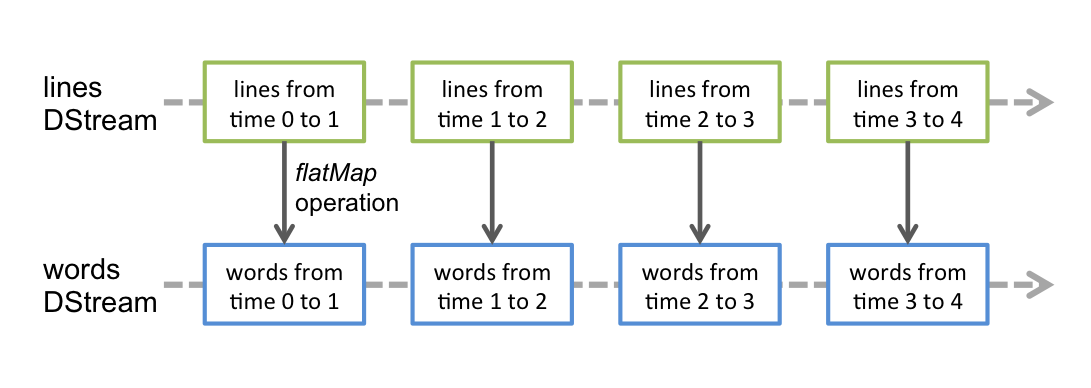
\includegraphics[scale=0.7]{streaming-dstream-ops}  
		\caption[Gambar mengubah{\it Data Stream} dari lines ke words]{mengubah{\it Data Stream} 				dari lines ke words} 
		\label{fig:processing-events relationship} 
		\end{figure}
	
		\textit{DStream} dapat dibuat dari sumber eksternal ataupun menggunakan hasil transformasi 				dari \textit{Dstream} lain. \textit{DStream} juga memiliki  \textit{Stateful 							transformations} yang bisa mengagregasi data pada seluruh interval yang ada. pembahasan 				tentang \textit{stateful transformation} akan dibahas lebih jelas di bab berikutnya.

		Untuk setiap sumber input, \textit{spark streaming} meluncurkan \textit{recievers} yang mana 		adalah \textit{task} yang berjalan pada eksekutor yang mengumpulkan data dari sumber input 				dan menyimpannya sebagai RDD. Selain menyimpan data, \textit{recievers} juga mereplikasi 				data ke eksekutor lain untuk mencapai \textit{fault-tolerance}. Data akan disimpan di memori 		eksekutor sama seperi \textit{cache} pada RDD. \textit{Receivers} juga bisa mereplikasi data 		ke HDFS. \textit{Streaming Context} pada \textit{driver} than secara periodik menjalankan 				\textit{Spark Jobs} untuk memproses data dan menggabungkannya dengan RDD sebelumnya.
  
		\begin{figure}[H] 
		\centering  
		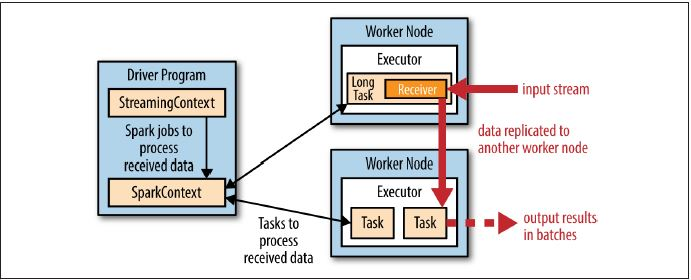
\includegraphics[scale=1]{spark-streaming-execution}  
		\caption[Gambar eksekusi{\it Spark Streaming} pada komponen \textit{Spark}]{eksekusi{\it 				Spark Streaming} pada komponen \textit{Spark}} 
		\label{fig:processing-events relationship} 
		\end{figure}

		\textit{Spark Streaming} memiliki sifat \textit{fault-tolerant} yang sama dengan 						\textit{Spark} untuk RDD selama replika input data masih tersedia. \textit{Spark Streaming} 			bisa mengkomputasi ulang setiap \textit{state} yang diturunkan dari \textit{lineage}suatu 				RDD dengan cara menjalankan kembali operasi yang memproses RDD tersebut. Biasanya, data yang 		diterima direplika dalam dua node sehingga \textit{spark streaming} bisa mentoleransi satu 				worker yang gagal. Namun, jika menggunakan \textit{lineage} penghitungan ulang bisa 					memerlukan waktu yang lama karena datanya telah dibuat duluan. Karena itu, \textit{Spark 				Streaming} menyediakan mekanisme yang disebut \textit{checkpointing} yang akan menyimpan 				state secara berkala ke suatu file system seperti HDFS. \textit{checkpointing} akan 					dijalankan setiap lima atau sepuluh \textit{batch}. Ketika terjadi ingin memperbaiki data 				yang gagal \textit{Spark Streaming} hanya perlu kembali ke \textit{checkpoint} paling baru.
		\\
		\textbf{Transformasi}\newline
		Transformasi pada \textit{Spark Streaming} dikelompokan menjadi dua yaitu; 								\textit{stateless} atau \textit{Stateful}:
		\begin{itemize}
			\item{ Pada transformasi \textit{stateless}, pemrosesan setiap batch tidak bergantung 					pada data di batch sebelumnya. Transformasi ini memiliki transformasi RDD seperti 						\texttt{map()},\texttt{reduce()}, dan \texttt{reduceByKey()}	
			}
	
			\item{Transformasi \textit{stateful} menggunakan data yang dihasilkan oleh 								\textit{batch} sebelumnya untuk menghitung hasil dari \textit{batch} saat ini. 							Transformasi ini memiliki \textit{sliding windows} dan bisa mengecek waktu pada seluruh 				interval.
	
			}
		\end{itemize}
		
		Walaupun setiap fungsi terlihat diterapkan ke pada seluruh aliran data. Namun, secara 			 		internal setiap \textit{DStream} tersusun dari beberapa RDD (\textit{batches}) dan setiap 		 		transformasi \textit{stateless} diterapkan secara terpisah untuk setiap RDD. Contohnya, 
		 \texttt{reduceByKey()} akan melakukan \textit{reduce} pada data pada setiap \textit{batch 		 		interval}. Untuk menggabungkan data pada seluruh interval diperlukan \textit{Stateful 			 		Transformation} 
	
	
		\item[]{\textbf{\textit{Stateful Transformation}}\newline
		\textit{Stateful Transformation} adalah sebuah operasi pada \textit{Dstream} yang bisa 					menelusuri waktu pada semua interval sehingga data pada \textit{batch} sebelumnya bisa 					digunakan untuk \textit{batch} saat ini.\newline
		\textit{Spark Streaming} memerlukan \textit{checkpointing} untuk bisa diaktifkan di 					\textit{streaming context} sebagai upaya menghindari kesalahan \textit{fault}. }
	
		\item[]{\textbf{\textit{Windowed Transformation}}\newline
		Transformasi ini menghitung hasil pada interval yang lebih lama dari \textit{streaming 					context} dengan menggabungkan beberapa \textit{batch} pada interval tertentu.
		pada transformasi \textit{windowing} ada tiga interval yang digunakan: \textit{batch, 					slide}, dan \textit{window interval}. \textit{Batch Interval} adalah seberapa sering 					suatu data diambil ke dalam \textit{Dstream}. Durasi dari batch interval sangat 						sebentar setengah sampai satu detik. \textit{Batch time} tidak berkorelasi dengan apa 					yang akan dianalisis nanti. \textit{Batch Interval} hanya mengambil data sebanyak dan 					secepat mungkin dari suatu sumber data. \newline
		
		\begin{figure}[H] 
		\centering  
		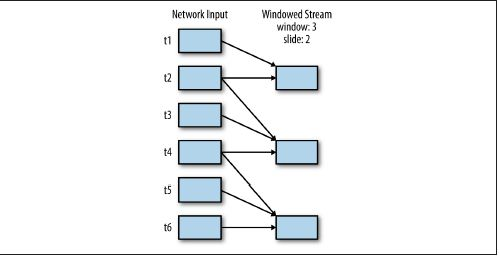
\includegraphics[scale=0.9]{windowing-streaming}  
		\caption[Gambar cara kerja \textit{Windowed Transformation}]{Gambar cara kerja 							\textit{Windowed Transformation}} 
		\label{fig:processing-events relationship} 
		\end{figure}
		}
		
		\textit{Slide Interval} adalah titik acuan seberapa sering suatu informasi ingin 						dikomputasi, dan \textit{Window Interval} adalah bagaimana \textit{Spark Streaming} 					melihat ke belekang setiap kali bertemu dengan \textit{slide Interval}.
		\newpage
		
		\item \textbf{Studi literatur mengenai Twitter API}\\
		{\bf Status :} Baru ditambahkan pada semester ini\\
		{\bf Hasil :}Twitter API adalah sekumpulan URL yang digunakan untuk mengakses data pada twitter tanpa melewati
antar muka web. URL akan digunakan sebagai parameter kode program nanti. data yang diambil pada twitter berupa objek. seperti contoh gambar:

\begin{figure}[H] 
	\centering  
	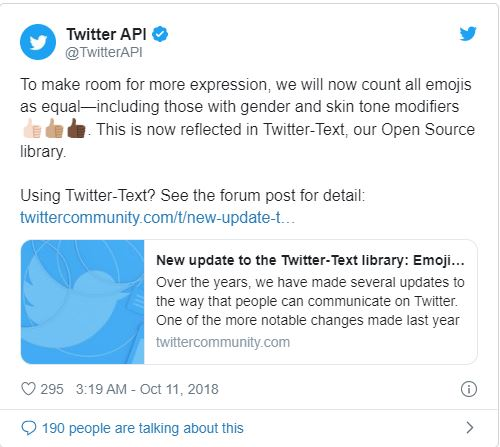
\includegraphics[scale=0.8]{twitter-object}  
	\caption[Gambar Twitter Object]{\textit{Twitter Object}} 
	\label{fig:Hadoop-home} 
\end{figure}

objek yang diakses akan disimpan dengan format JSON. Objek terdiri dari informasi-informasi yang membangun tweet seperti; tanggal berapa suatu tweet dibuat, id twitter yang menunggah tweet tersebut, isi pesan yang diunggah oleh pengguna(status), informasi pengguna itu sendiri, dan entitas luar yang ikut di dalam suatu tweet seperti link url atau mention. Berikut adalah contoh format JSON yang membangun suatu Tweet:

\begin{figure}[H] 
	\centering  
	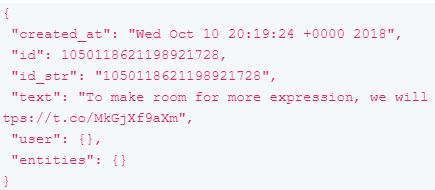
\includegraphics[scale=1]{twitterJSON}  
	\caption[Gambar Twitter Object]{\textit{Twitter Object JSON}} 
	\label{fig:Hadoop-home} 
\end{figure}

Informasi tentang pengguna terdiri dari beberapa objek lagi.Objek yang dimuat berupa id user, nama,
lokasi, url, deskripsi, status verifikasi, jumlah follower, jumlah following, dan lokasi.
 
\begin{figure}[H] 
	\centering  
	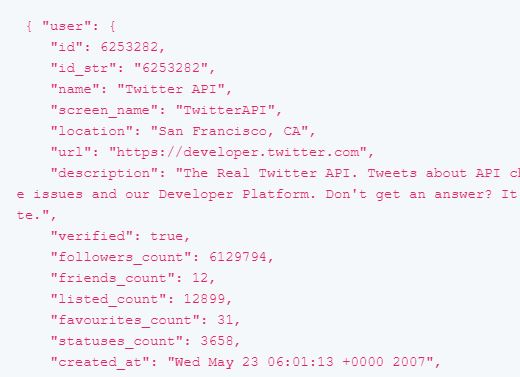
\includegraphics[scale=1]{userObject}  
	\caption[Gambar Twitter Object]{\textit{User Object JSON}} 
	\label{fig:Hadoop-home} 
\end{figure}

Namun dari beberapa banyak informasi yang terdapat pada twitter seseorang tidak semuanya bisa diakses hal ini bergantung ke pada kebijakan dari twitter dan persetujuan dari user. salah satu contohnya adalah lokasi seseorang. Lokasi seseorang hanya bisa diakses ketika user bersedia untuk menampilkan lokasi tersebut.
		
		\item \textbf{Studi literatur mengenai Kafka}\\
		{\bf Status :} Baru ditambahkan pada semester ini\\
		{\bf Hasil :}Sebelum membahas Kafka, penting untuk mengerti tentang sistem pengiriman 					\textit{publish/messaging} dan mengapa konsep ini sangat penting. \textit{publish/subscribe 			messaging} adalah \textit{pattern} yang dicirikan oleh pengirim \textit{publisiher} tidak 				langsung mengirimkannya ke penerima. Tetapi, pengirim mempublikasikan data yang dimiliki ke 			sebuah sistem lain yang disebut \textit{broker}, sebuah titik sentral di mana suatu pesan 				selalu diunggah. Sehingga penerima pesan bisa langsung mengikuti perkembangan data dan 					informasi yang dimiliki \textit{publisher} di broker. Penerima disebu \textit{Subscriber}.
		
		\begin{figure}[H] 
		\centering  
		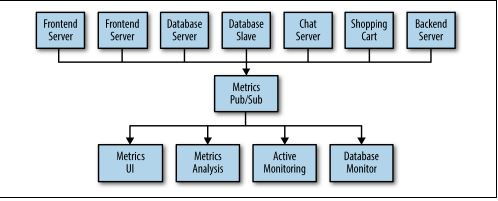
\includegraphics[scale=1]{pubsub}  
		\caption[Gambar Publisher/Subscriber]{\textit{Publisher/Subscriber}} 
		\label{fig:pub-sub} 
		\end{figure}

		seperti gambar di atas semua server mengirimkan data ke broker \textit{metrics} dan sistem-				sistem yang ingin memilki data yang ingin diakses harus diintegrasikan dengan broker. 					Sistem-sistem tersebut mengikuti perkembangan dan perubahan data yang terjadi melalui broke 			(subscribe).
		
		\textbf{Pengertian Kafka} \newline
		kafka adalah sebuah sistem pengriman data \textit{Publish/subscribe} yang didesain untuk 				menyelesaikan masalah yang sering disebut dengan \textit{distributed commit log} yang mana 				suatu \textit{filesystem} atau database didesain untuk menyediakan data rekord-rekord yang 				disimpan dengan lama dan bisa diakses kembali secara berkala pada sistem yang stabil. Data 				pada kafka disimpan dengan lama dan terurut. Berikut dalah komponen-komponen dari kafka:
		
		\textbf{Messages and Batches} \newline
		Satuan data di kafka disebut dengan \textit{message}. \textit{Message} hampir sama seperti 				\textit{row} atau \textit{rekord}. Sebuah \textit{message} adalah array dari sekumpulan 				bytes karena itu \textit{message} pada kafka tidak memiliki format spesifik atau arti bagi 				kafka. Suatu \textit{message} bisa memiliki metadata yang disebut dengan \textit{key}. Untuk 		lebih efisien semua \textit{messages} ditulis pada \textit{batch}. \textit{batch} adalah 				sekumpulan pesan yang diproduksi oleh topik dan partisi yang sama.
		
		\textbf{Schemas}\newline
		Kakfa mengetahui \textit{message} adalah sebuah \textit{array of bytes}. Sehingga kafka 				membutuhkan skema atau struktur yang diterapkan pada pesan sehinggga bisa mudah dimengerti. 			Ada banyak cara untuk menerapkan skema tergantung kebutuhan aplikasi. Contoh dari skema bisa 		berbentuk JSON atau XML sehingga manusia bisa membaca pesan yang ada pada kafka.
		
		\textbf{Topics}\newline
		\textit{Message} pada kafka disebut sebagai \textit{topics}. \textit{Topics} adalah sebuah 				kategori atau sebuah nama \textit{feed} dimana suatu rekord dipublikasi. Analoginya, topik 				adalah tabel basis data atau suatu folder di filesystem. Suatu rekord bisa disimpan di 					folder atau basis data dengan identifikasi pengenal.
		
		\textit{Message} pada kafka disebut sebagai \textit{topics}. \textit{Topics} adalah sebuah 				kategori atau sebuah nama \textit{feed} dimana suatu rekord dipublikasi. Analoginya, topik 				adalah tabel basis data atau suatu folder di filesystem. Suatu rekord bisa disimpan di 					folder atau basis data dengan identifikasi pengenal.

		\begin{figure}[H] 
		\centering  
		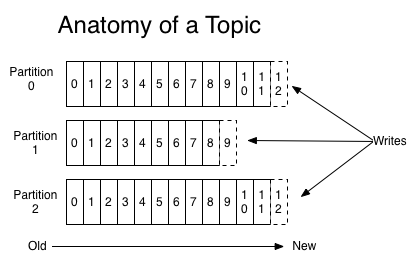
\includegraphics[scale=0.7]{kafkatopic}  
		\caption[Gambar Topic pada Kafka]{\textit{Topic pada kafka}} 
		\label{fig:kafka-topic} 
		\end{figure}
		
		Setiap partisi adalah sebuah sekuensi yang terurut, tidak bisa diubah-ubah 								\textit{immutable} yang terus ada pada \textit{commit log}. Setiap rekord pada p						\textit{partition} diberi tanda dengan nomer sekuensial yang disebut offset yang menandai 				rekord secara unik. Partition adalah tempat dimana topic disimpan.

		Klaster pada kafka akan terus menyimpan topic terlepas topik itu digunakan atau tidak selama 		waktu yang telah ditentukan \textit{(retention period)}. Contoh jika suatu \textit{retention 		period} pada topic diatur menjadi 2 hari maka topic tersebut akan ada selama dua hari dan 				tidak bisa dihapus pada interval waktu itu. Sehingga setiap \textit{subscriber} masih bisa 				mengakses data tersebut. Setelah itu baru dihapus.

		\begin{figure}[H] 
		\centering  
		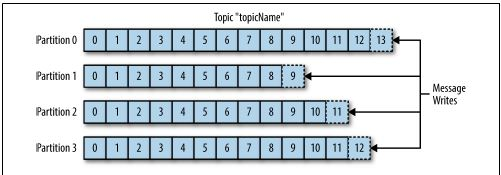
\includegraphics[scale=1]{streamtopic}  
		\caption[Gambar stream topic]{\textit{stream topic}} 
		\label{fig:kafka-stream} 
		\end{figure}

		Begitu juga dengan \textit{data stream}. Pada kafka, \textit{Data Stream} dianggap sebagai 				satu topic terlepas dari banyak partisi. Sebagai contoh keempat partisi pada gambar di atas 			masih disebut sebagai satu stream.
		
		\textbf{Producers and Consumers}\newline
		Pengguna yang menggunakan sistem kafka disebut dengan klien. Ada dua tipe kline 						\textit{producer} dan \textit{consumer}. Bisa juga kakfa diintegrasikan dengan sistem API 				lain. Tugas dari \textit{producer} adalah membuat \textit{membuat message} dan mengirimnya 				ke \textit{topic} tertentu pada broker. \textit{Consumer} adalah yang membaca pesan degan 				cara mengakses topic-topic tertentu pada broker.
		
		\textbf{Broker}\newline
		Sebuah kafka server disebut dengan broker. Sebuah broker menerima pesan dari 							\textit{producer} memberi \textit{offset} pada pesan tersebut dan menyimpannya pada sebuah 				disk. Broker juga berinteraksi dengan \textit{consumer} ketika konsumer meminta akses pada 				suatu partisi dan membalas \textit{consumer} dengan pesan yang diinginkan dan ada di disk.
 
 		\begin{figure}[H] 
		\centering  
		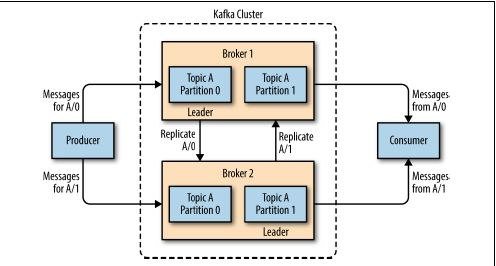
\includegraphics[scale=1]{replikasibroker}  
		\caption[Gambar Kafka Broker]{Kafka Broker} 
		\label{fig:kafka-broker} 
		\end{figure}

 		\textit{Broker} dirancang untuk berjalan pada klaster. Dari rangkaian \textit{broker} pada 				klaster
 		satu \textit{broker} akan bertindak sebagai \textit{controller} yang dipilih secara otomatis 		dan berfungsi untuk mengatur operasi administratif seperti; menentukan partisi mana topic 				akan disimpan atau mengawasi jika terjadi \textit{failure} pada broker lain. Sebuah partisi 			bisa disimpan pada dua broker secara bersamaan.
 		
 		\item \textbf{Konfigurasi TCP Socket}\\
		{\bf Status :} Sudah ada sejak perencanaan skripsi\\
		{\bf Hasil :}Sumber data TCP Socket tidak perlu diinstalasi terlebih dahulu karena tidak ada 		interverensi dari pihak ketiga yaitu sang penyedia data. TCP socket langsung bisa menerimas 			data dengan mengakses port lokal dan akan langsung terintegrasi dengan IP address dan port 				yang kita miliki. Mengkonfigurasikan TCP Socket hanya perlu menyediakan sebuah port kosong 				yang nantinya akan digunakan data untuk masuk. Tetapi, konfigurasi pada kode program masih 				diperlukan.
		
		\item \textbf{Mengintegrasikan \textit{spark streaming} dengan twitter API}\\
		{\bf Status :} Ada sejak rencana kerja skripsi.\\
		{\bf Hasil :} Sebelum mendapatkan hak untuk mengakses Twitter API, user perlu melakukan 				pendaftaran ke pihak twitter untuk menjadi \textit{developer account} terlebih dahulu. Akan 			muncul survei yang menanyakan tentang privasi data pengguna twitter.Pertanyaan paling umum 				adalah data yang didapatkan akan digunakan untuk apa. Untuk kasus skripsi ini, data akan 				digunakan untuk mempelajari Spark Streaming. Berikut adalah cara membuat API Setelah 					dikonfirmasi menjadi \textit{developer account}:

	\begin{enumerate}
		\item Membuat Aplikasi yang akan digunakan sebagai API.
		\item Mengisi keterangan dan informasi tentang aplikasi tersebut
		\item Menggunakan keys dan tokens yang didapatkan yang akan digunakan untuk integrasi dengan 		Spark Streaming
	\end{enumerate} 

	keys dan tokens yang didapatkan adalah beberapa nomer seri yang disbut \textit{Consumer API} dan 	\textit{Access token}. 
	Nomor seri ini yang nantinya akan jadi parameter bagi kode program untuk mengakses Aplikasi yang 	telah kita buat. 
	Nomor seri ini bersifat rahasia jadi tidak boleh tersebar ke pihak lain karena seseorang bisa 			mengakses Aplikasi pengumpul data yang telah kita buat. 
	Berikut contoh gambar dari key dan tokens:

		\begin{figure}[H] 
		\centering  
		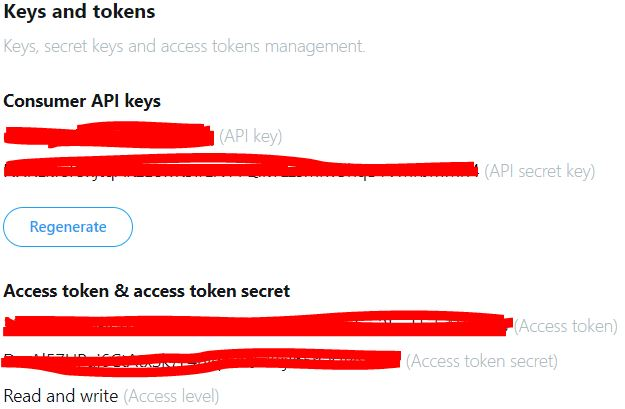
\includegraphics[scale=0.8]{TwitterTokens}  
		\caption[Gambar Twitter Tokens]{Gambar Token yang digunakan sebagai parameter} 
		\label{fig:Hadoop-home} 
		\end{figure}

		Parameter keys dan token nantinya akan dimuat dalam \texttt{twitterAuth.txt}. 
		File tersebut akan dijadikan sebagai otentikasi untuk mengakses data yang ada di Twitter.
			
		\item \textbf{Integrasi dengan Kafka}\\
		{\bf Status :} Sudah ada sejak perencanaan skripsi\\
		{\bf Hasil :}kafka adalah sebuah sistem pengriman data \textit{Publish/subscribe} yang 					didesain untuk menyelesaikan masalah yang sering disebut dengan \textit{distributed commit 				log} yang mana suatu \textit{filesystem} atau database didesain untuk menyediakan data 					rekord-rekord yang disimpan dengan lama dan bisa diakses kembali secara berkala pada sistem 			yang stabil. Kafka akan menjadi Input Sources bagi spark streaming. 

		Untuk sistem \textit{standalone} port zookeper bisa diatur. tetapi port default adalah 2181. 		Untuk menjalankan Zookeper lakukan perintah \texttt{zkserver}. Sebelum menginstal broker 				pastikan zookeeper berjalan terlebih dahulu. Setelah zookeeper berhasil terinstal. perlu 				menjalankan broker karena \textit{consumer} dan \textit{producer} membutukan \textit{broker} 		untuk bisa diinstal dan saling berkomunikasi. perintah untuk menjalankan broker: \path{.\bin			\windows\kafka-server-start.bat .\config\server.properties}. Setelah menjalankan broker dan 			zookeeper, membuat \textit{topics} untuk kafka.

		\begin{figure}[H] 
		\centering  
		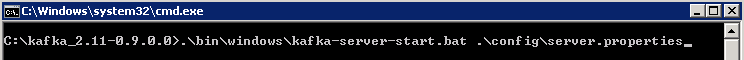
\includegraphics[scale=0.8]{serverkafka}  
		\caption[Gambar menjalankan server]{menjalankan server} 
		\label{fig:topic-run} 
		\end{figure}

		\textit{Topics} yang dibuat dengan nama \"Test\" dan akan direplika sebanyak satu kali jika 			\textit{standalone}. Jika memiliki klaster lebih dari satu maka bisa mereplikasi lebih dari 			satu dan replikasi tersebut digunakan sebagai \textit{backup} jika terjadi kegagalan. Topik 			dapat dibuat dengan perintah: \path{kafka-topics.bat --create --zookeeper localhost:2181 --				replication-factor 1 --partitions 1 --topic test}

		\begin{figure}[H] 
		\centering  
		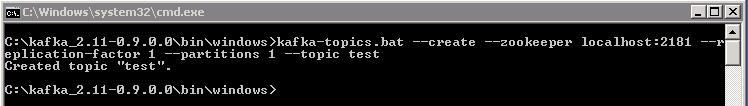
\includegraphics[scale=0.8]{topickafka}  
		\caption[Gambar menjalankan topic]{menjalankan topic} 
		\label{fig:topic-run} 
		\end{figure}

		Untuk mengetes apakah suatu server sudah jalan perlu dilakukan pengecekan dengan membuat 				broker \textit{producer} dan \textit{consumer}. Untuk menjalankan \textit{producer}, lakukan 		perintah \path{kafka-console-producer.bat --broker-list localhost:9092 --topic test} dan 				untuk menjalankan \textit{consumer} lakukan perintah \path{kafka-console-consumer.bat --				zookeeper localhost:2181 --topic test}. Jika berhasil \textit{consumer} dan 							\textit{producer} akan saling terhubung.

		\begin{figure}[H] 
		\centering  
		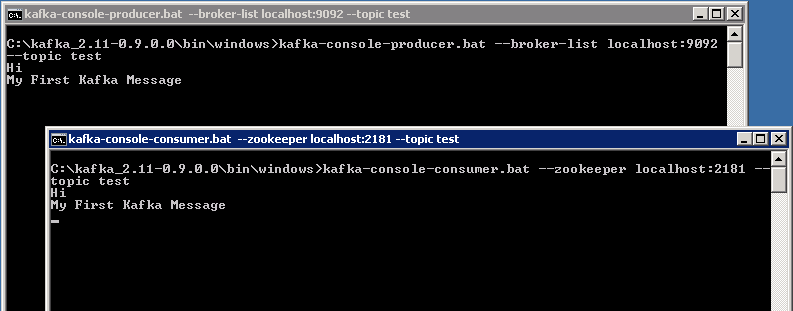
\includegraphics[scale=0.8]{10}  
		\caption[Gambar \textit{consumer}-\textit{producer}]{\textit{consumer}-\textit{producer}} 
		\label{fig:topic-run} 
		\end{figure}
		
		\item \textbf{Mengeksplorasi dan Menganalisis data yang didapat dari TCP Socket}\\
		{\bf Status :} Ada sejak rencana kerja skripsi.\\
		{\bf Hasil :}Studi Eksplorasi dilakukan dengan mencoba mengumpulkan data dari salah satu 				penyedia data yaitu TCP Socket. karena ini berupa simulasi, maka file input data web logs 				akan diunduh terlebih dahulu disimpan pada sebuah file \texttt{accesslog.txt}. Lalu 					menggunakan perintah \texttt{ ncat -lk 9999 < accesslog.txt} yang artinya \texttt{ncat} akan 		memasukan data ke TCP port 9999 satu demi satu seolah-olah data yang masuk berupa aliran 				data.

		\begin{figure}[H] 
		\centering  
		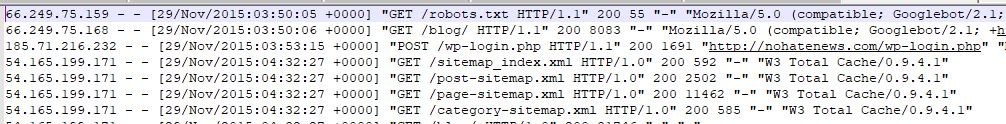
\includegraphics[scale=0.8]{ncatinput}  
		\caption[Gambar File input]{File input} 
		\label{fig:Output-Log-Parser} 
		\end{figure}

		Data yang akan dianalisis adalah simulasi web logs data stream yang datang dari aktivitas 				suatu website. Eksplorasi ini akan menghitung seberapa sering suatu file dibuka oleh 					pengguna. Berikut cara membuat spark streaming. Contoh Gambar
  
		\begin{figure}[H] 
		\centering  
		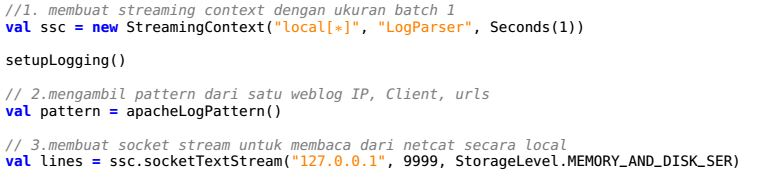
\includegraphics[scale=0.7]{urlcountersetup}  
		\caption[Gambar pengaturan spark streaming]{pengaturan spark streaming} 
		\label{fig:Output-Log-Parser} 
		\end{figure}

		\begin{figure}[H] 
		\centering  
		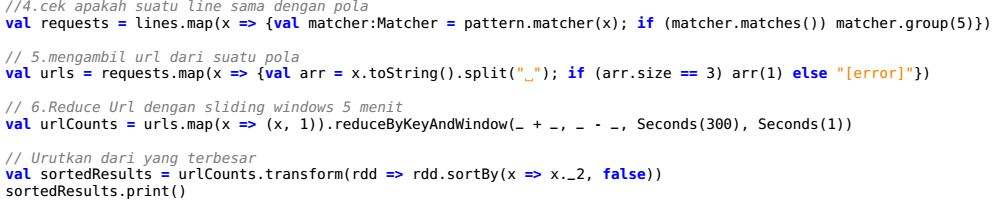
\includegraphics[scale=0.7]{urlcountertransform}  
		\caption[Gambar perhitungan url]{perhitungan url} 
		\label{fig:Output-Log-Parser} 
		\end{figure}

		Spark streaming dibuat dengan menentukan ukuran batch interval (Streaming Context) selama 1 			detik. Pada interval 1 detik Spark Streaming akan mengambil data yang dihasilkan pada 					interval teresbut. lalu, menggunakan metode dari library ambil web log yang hanya mengikuti 			pola saja. Jadi, jika ada data lain yang masuk tapi tidak berbentuk web logs akan diabaikan. 		Menghubungkan batch inteval dengan socket stream untuk mendapatkan data. Mengambil url file 			dari potongan web logs tersebut contoh \texttt{apachepb.gif}.Menghitung dengan 							ReduceByKeyAndWindow artinya hitung berapa banyak jumlah url pada key dan windows yang sama. 		Terakhir urutkan url dari yang memiliki hit paling banyak dan tampilkan 10 hasil terbaik. 				Contoh Gambar

		\begin{figure}[H] 
		\centering  
		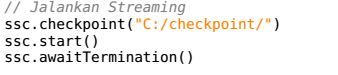
\includegraphics[scale=0.8]{sparkstreamingrun}  
		\caption[Gambar File input]{Menjalankan Spark Streaming} 
		\label{fig:Output-Log-Parser} 
		\end{figure}

		Terakhir jalankan spark streaming yang telah dibuat. \texttt{ssc.awaitTermination()} 					menyatakan bahwa proses pengambilan data tidak akan berhenti sampai ada perintah dari user. 			Contoh Gambar

		\begin{figure}[H] 
		\centering  
		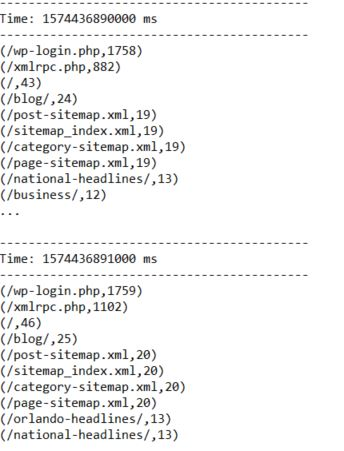
\includegraphics[scale=0.8]{parserOutput}  
		\caption[Gambar Output Web Log]{Output Web log} 
		\label{fig:Output-Log-Parser} 
		\end{figure}

		hasil dari eksekusi program tersebut adalah batch dengan interval yang telah kita atur dan 				pada tiap batch interval tersebut berisi hasil komputasi 10 file yang paling sering diakses. 		Dari hasil dapat disimpulkan pada batch pertama file yang paling sering diakses dalah 					\texttt{wp-login.php}

		\item \textbf{Mengeksplorasi dan Menganalisis data yang didapat dari Twitter API}\\
		{\bf Status :} Ada sejak rencana kerja skripsi.\\
		{\bf Hasil :}Perangkat lunak yang akan dikembangakan adalah perangkat lunak spark. Perangkat lunak digunakan untuk mengambil data dengan sistem \textit{spark streaming} dan melakukan analisis sederhana secara \textit{real-time}. Program saat ini akan menghitung jumlah hashtag terbanyak pada lima menit terakhir. set data yang akan diambil oleh \textit{spark streaming} bersifat \textit{real-time}. Hal ini dilakukan dengan mengintegrasikan \textit{spark streaming} dengan sistem eksternal yang meyediakan data melalui API. Untuk kasus ini akan digunakan data yang berasal dari twitter.\\
Data yang didapatkan dari twitter adalah berupa \textit{twitter object} dalam format JSON. Data twitter akan diambil selama 5 menit dan keluaran akan berupa pasangan key value yang bernilai (hashtag,value).Untuk membuat sistem penghitung hashtag bekerja, harus membuat batch window yang nanti akan diintegrasikan dengan Twitter. Lalu Setiap Objek akan dipetakan dan hanya diambil statusnya saja karena informasi hashtag terletak pada status seseorang. Status yang telah didapat akan dipetakan lagi dan dipisahkan perkata. Lalu fungsi filter akan dipanggil dan kita hanya mengambil simbol \# yang merepresentasikan \textit{Hashtag}. Hashtag akan dipetakan lagi dengan map hingga berisi pasangan key value. dengan nilai key adalah hashtag dan value adalah jumlahnya. Lalu akan dilakukan \textit{reduce} berdasarkan nilai key dan batch window yang sama. Atur ukuran window menjadi 5 menit.

		\begin{figure}[H] 
		\centering  
		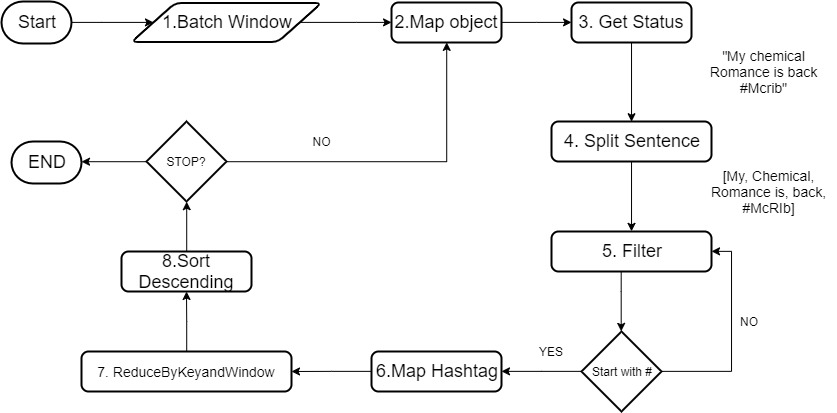
\includegraphics[scale=0.5]{HashtagFlow}  
		\caption[Twitter Obejct]{Flowchart diagram analisis hashtag} 
		\label{fig:processing-events relationship} 
		\end{figure}
		
\begin{enumerate}
		\item[1.]Membuat batch window berukuran satu detik. setiap satu detik akan menangkap
		objek-objek dari twitter.
		\item[2.]Memetakan setiap objek menjadi statusnya saja artinya dari seluruh objek tweet
		seperti nama atau location yang kita ambil hanya perkataan yang diposting oleh user 					saja.
		\item[3.]Mengambil statusnya satu per satu
		\item[4.]Membagi kalimat berdasarkan spasi lalu menyimpannya di array
		\item[5.]Filter setiap elemen pada array jika elemen pada array tidak sama
		dengan \# maka akan terus melakukan filter sampai status pada batch ini habis
		\item[6.]memetakan hashtag menjadi $[key,value] =>[hashtag,1]$
		\item[7.]melakukan reduce penjumlahan berdasarkan key dan windows yang sama.
		\item[8.]Mengurutkan hashtag berdasarkan value dari nilai yang paling tinggi.
		\item[9.]Jika program sudah diberhentikan maka tidak akan mengumpulkan objek lagi.
		Tetapi, jika tidak akan terus berlanjut.
\end{enumerate}
		
		berikut kode pengerjaan dari perhitungan hashtag selama lima menit terakhir:
		
\begin{lstlisting}[showstringspaces=false,language=Scala]
							
// Setting twitter Credentials
setupTwitter()
    
//setup streaming context ukuran 1 detik
val ssc = new StreamingContext("local[*]", "PopularHashtags", Seconds(1))
    
// hapus spam selain error
setupLogging()

// Membuat Dstream dengan Streaming context
val tweets = TwitterUtils.createStream(ssc, None)
    
// ambil status
val statuses = tweets.map(status => status.getText())
    
// ambil setiap kata
val tweetwords = statuses.flatMap(tweetText => tweetText.split(" "))
    
// filter yang bukan hashtag
val hashtags = tweetwords.filter(word => word.startsWith("#"))
    
// Map setiap hastag menjadi key value (hashtag,1)
val hashtagKeyValues = hashtags.map(hashtag => (hashtag, 1))
    
//Hitung hashtag perdetik dengan sliding window selama 5 menit
val hashtagCounts = hashtagKeyValues.reduceByKeyAndWindow( (x,y) => x + y, 
			(x,y) => x - y,Seconds(300), Seconds(5))
    
// Sort berdasarkan banyak hashtag
val sortedResults = hashtagCounts.transform(rdd => rdd.sortBy(x => x._2, false))
    
// Print the top 10 dan save di HDFS
sortedResults.saveAsTextFiles("hdfs:
		//localhost:50071/Twitter/Hashtag/Output1", "txt")
sortedResults.print
    
ssc.checkpoint("C:/checkpoint/")
ssc.start()
ssc.awaitTermination()


\end{lstlisting}
		
	hasil keluaran :
	
		\begin{figure}[H] 
		\centering  
		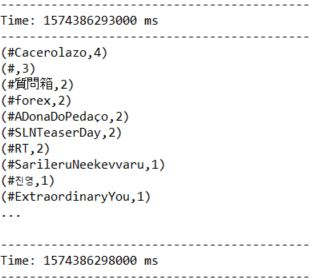
\includegraphics[scale=1]{outputTwitter}  
		\caption[Twitter Obejct]{Hasil perhitungan Hashtag} 
		\label{fig:processing-events relationship} 
		\end{figure}
	
	
		\item \textbf{Menulis Dokumentasi Skripsi}\\
		{\bf Status :} baru ditambahkan pada semester ini\\
		{\bf Hasil :}Penulisan skripsi baru selesai Bab I, Bab II, Bab III dan sebagian Bab IV 
		

\end{enumerate}


\section{Pencapaian Rencana Kerja}
Langkah-langkah kerja yang berhasil diselesaikan dalam Skripsi 1 ini adalah sebagai berikut:
\begin{enumerate}
\item Studi Literatur mengenai \textit{Big Data} dan \textit{Big Data Stream}
\item Studi Literatur mengenai teknik stream processing
\item Studi literatur mengenai pola teknik pemrosesan stream processing
\item Studi literatur arsitektur Stream Processing
\item Studi literatur mengenai sistem terdistribusi Spark
\item Studi Literatur Spark: Arsitektur Spark
\item Studi literatur mengenai Spark Streaming
\item Mengintegrasikan spark streaming dengan twitter API
\item Mengintegrasikan spark streaming dengan TCP socket
\item Mengintegrasikan spark streaming dengan Kafka
\item Mengeksplorasi dan Menganalisis data yang disumulasikan di TCP socket
\item Mengeksplorasi dan Menganalisis data yang didapat dari Twitter API
\item Menulis Dokumentasi skripsi Bab I dan Sebagian Bab II, Bab III, dan Bab IV
\end{enumerate}


\section{Kendala yang Dihadapi}
%TULISKAN BAGIAN INI JIKA DOKUMEN ANDA TIPE A ATAU C
Kendala - kendala yang dihadapi selama mengerjakan skripsi :
\begin{itemize}
	\item Kesulitan meng-instal environment di PC.
	\item Banyak tugas dari mata kuliah lain
	\item Sering ada versi yang tidak saling cocok.
	\item terlalu banyak environment yang di-instal
	
\end{itemize}

\vspace{1cm}
\centering Bandung, \tanggal\\
\vspace{2cm} \nama \\ 
\vspace{1cm}

Menyetujui, \\
\ifdefstring{\jumpemb}{2}{
\vspace{1.5cm}
\begin{centering} Menyetujui,\\ \end{centering} \vspace{0.75cm}
\begin{minipage}[b]{0.45\linewidth}
% \centering Bandung, \makebox[0.5cm]{\hrulefill}/\makebox[0.5cm]{\hrulefill}/2013 \\
\vspace{2cm} Nama: \pembA \\ Pembimbing Utama
\end{minipage} \hspace{0.5cm}
\begin{minipage}[b]{0.45\linewidth}
% \centering Bandung, \makebox[0.5cm]{\hrulefill}/\makebox[0.5cm]{\hrulefill}/2013\\
\vspace{2cm} Nama: \pembB \\ Pembimbing Pendamping
\end{minipage}
\vspace{0.5cm}
}{
% \centering Bandung, \makebox[0.5cm]{\hrulefill}/\makebox[0.5cm]{\hrulefill}/2013\\
\vspace{2cm} Nama: \pembA \\ Pembimbing Tunggal
}
\end{document}

